\documentclass[12pt]{article}

\usepackage{fullpage}
\usepackage{graphicx, rotating, booktabs} 
\usepackage{times}
\usepackage{fbb} 
\usepackage{natbib} 
\usepackage{indentfirst} 
\usepackage{setspace}
\usepackage{grffile} 
\usepackage{hyperref}
\usepackage{adjustbox}
\usepackage{multirow} 
\usepackage{amsmath}
\usepackage[labelfont={bf},textfont=it,labelsep=period]{caption}
\setcitestyle{aysep{}}
\usepackage{sectsty}
% for the big table
\usepackage{afterpage}
\usepackage{array}
\usepackage{lscape}
\usepackage{longtable}
\usepackage{float}
\usepackage{afterpage}
\sectionfont{\Large}
\subsectionfont{\noindent\large\textit}
\subsubsectionfont{\normalsize}


\singlespace
\title{\textbf{Appendix: Arms and Electoral Influence: Arms Deals with Autocracies, Defense Contracting and U.S. Presidential Elections}}
%\author{Joshua Alley} 
\date{}

\bibliographystyle{apsr}

\begin{document}

\maketitle 

\singlespace 

\tableofcontents

\bigskip





\section{Arms Deals Count Model Check}

In this section, I check the hurdle Poisson models of U.S. arms deals in three steps. 
First, I show similar patterns in raw data. 
Second, I demonstrate that two different Poisson model specifications and a zero-inflated Poisson model give similar inferences to the hurdle Poisson models in the manuscript. 
Finally, I use posterior predictive checks to show that a hurdle Poisson outcome likelihood fits the observed data best. 


\subsection{Raw Data}

The pattern of increasing arms deals with autocratic allies as presidential elections approach is evident in raw data.
\autoref{fig:deals-democ-raw} plots the number of arms deals per country after dividing state-year observations based on years to a presidential election, four quartiles of polyarchy, and whether a country is U.S. ally.
Autocratic U.S. allies average more than one additional deal in election years than in years immediately after an election. 
More democratic allies receive more arms deals than non-allied states, but deals with these countries do not track the electoral cycle. 


\begin{figure}[htpb]
	\centering
		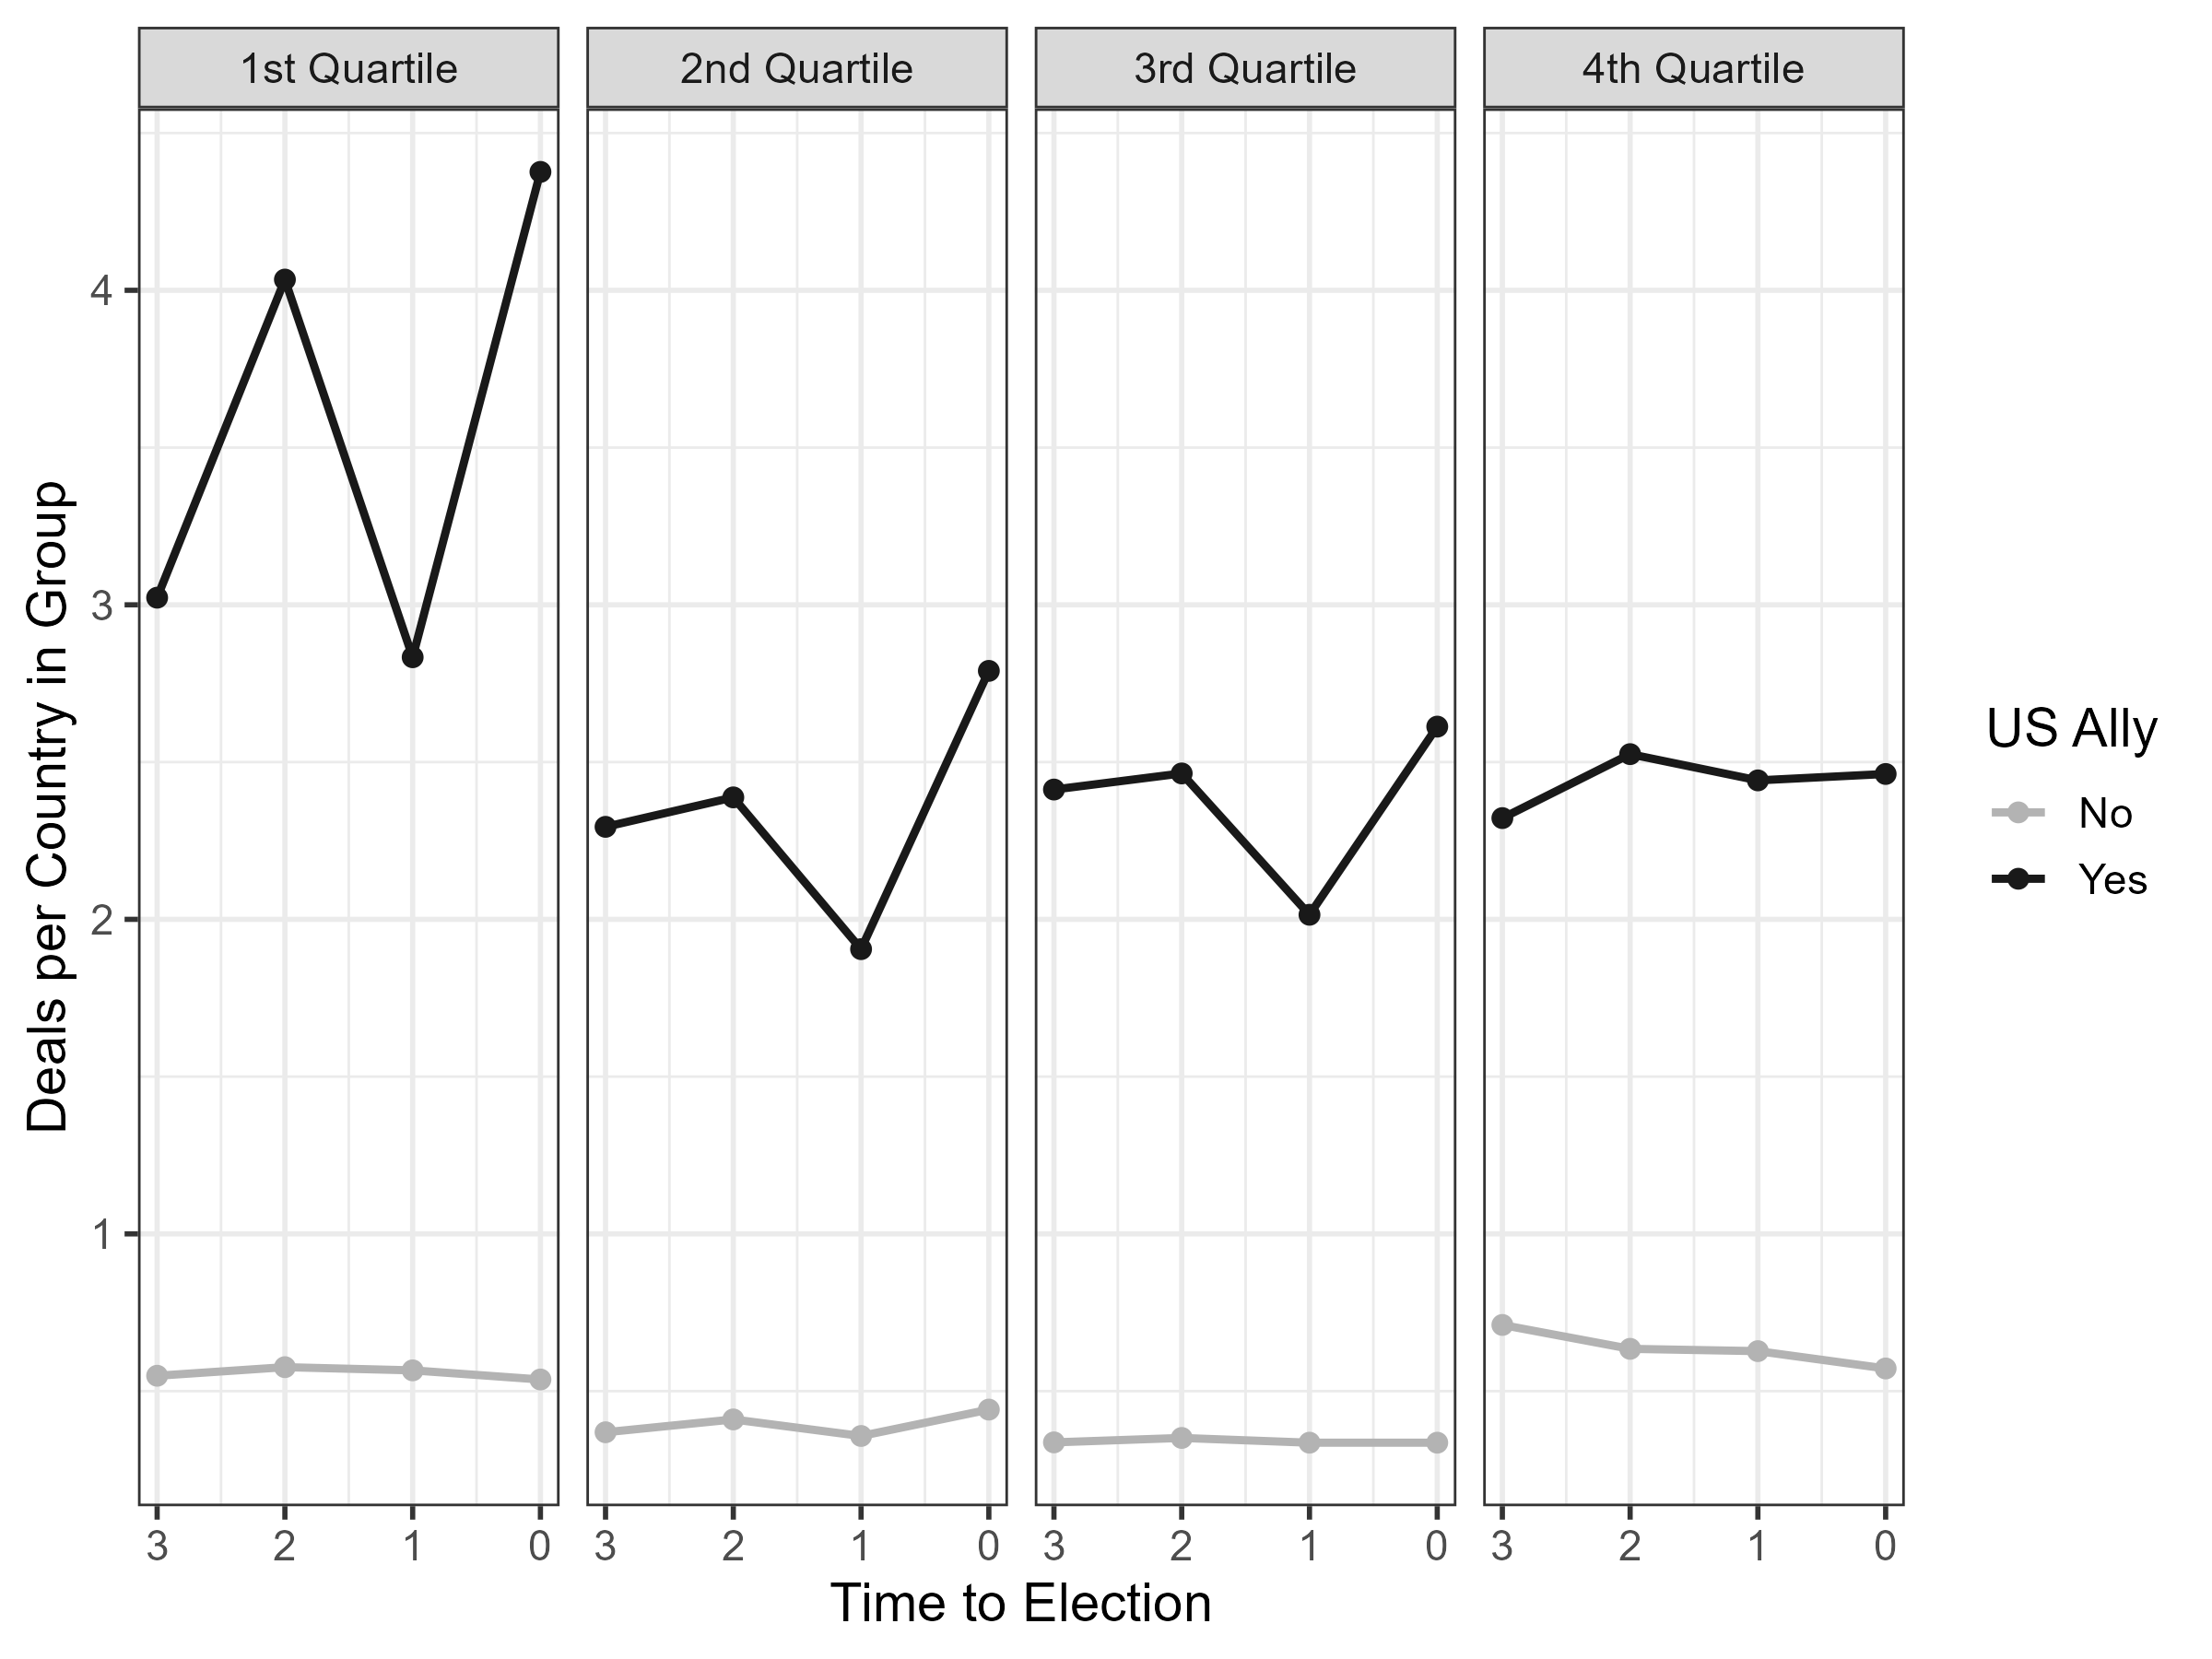
\includegraphics[width=0.95\textwidth]{deals-democ-raw.png}
	\caption{Average arms deals with the United States per country in each quartile of democracy throughout U.S. presidential election cycles. Colors divide states based on whether they are U.S. allies.}
	\label{fig:deals-democ-raw}
\end{figure}


\subsubsection{General Arms Deal Cycles}

In addition to the raw data, arms deal cycles are apparent even without interacting the time to presidential election measure with polyarchy.
I plot predicted arms deals as a function of years to a presidential election from a model that does not interact the election timing variable with anything else in \autoref{fig:elec-pred-deals}. 
Because it averages across all states, the increase of .05 deals across a presidential election cycle is small but distinguishable from zero. 


\begin{figure}[htpb]
	\centering
		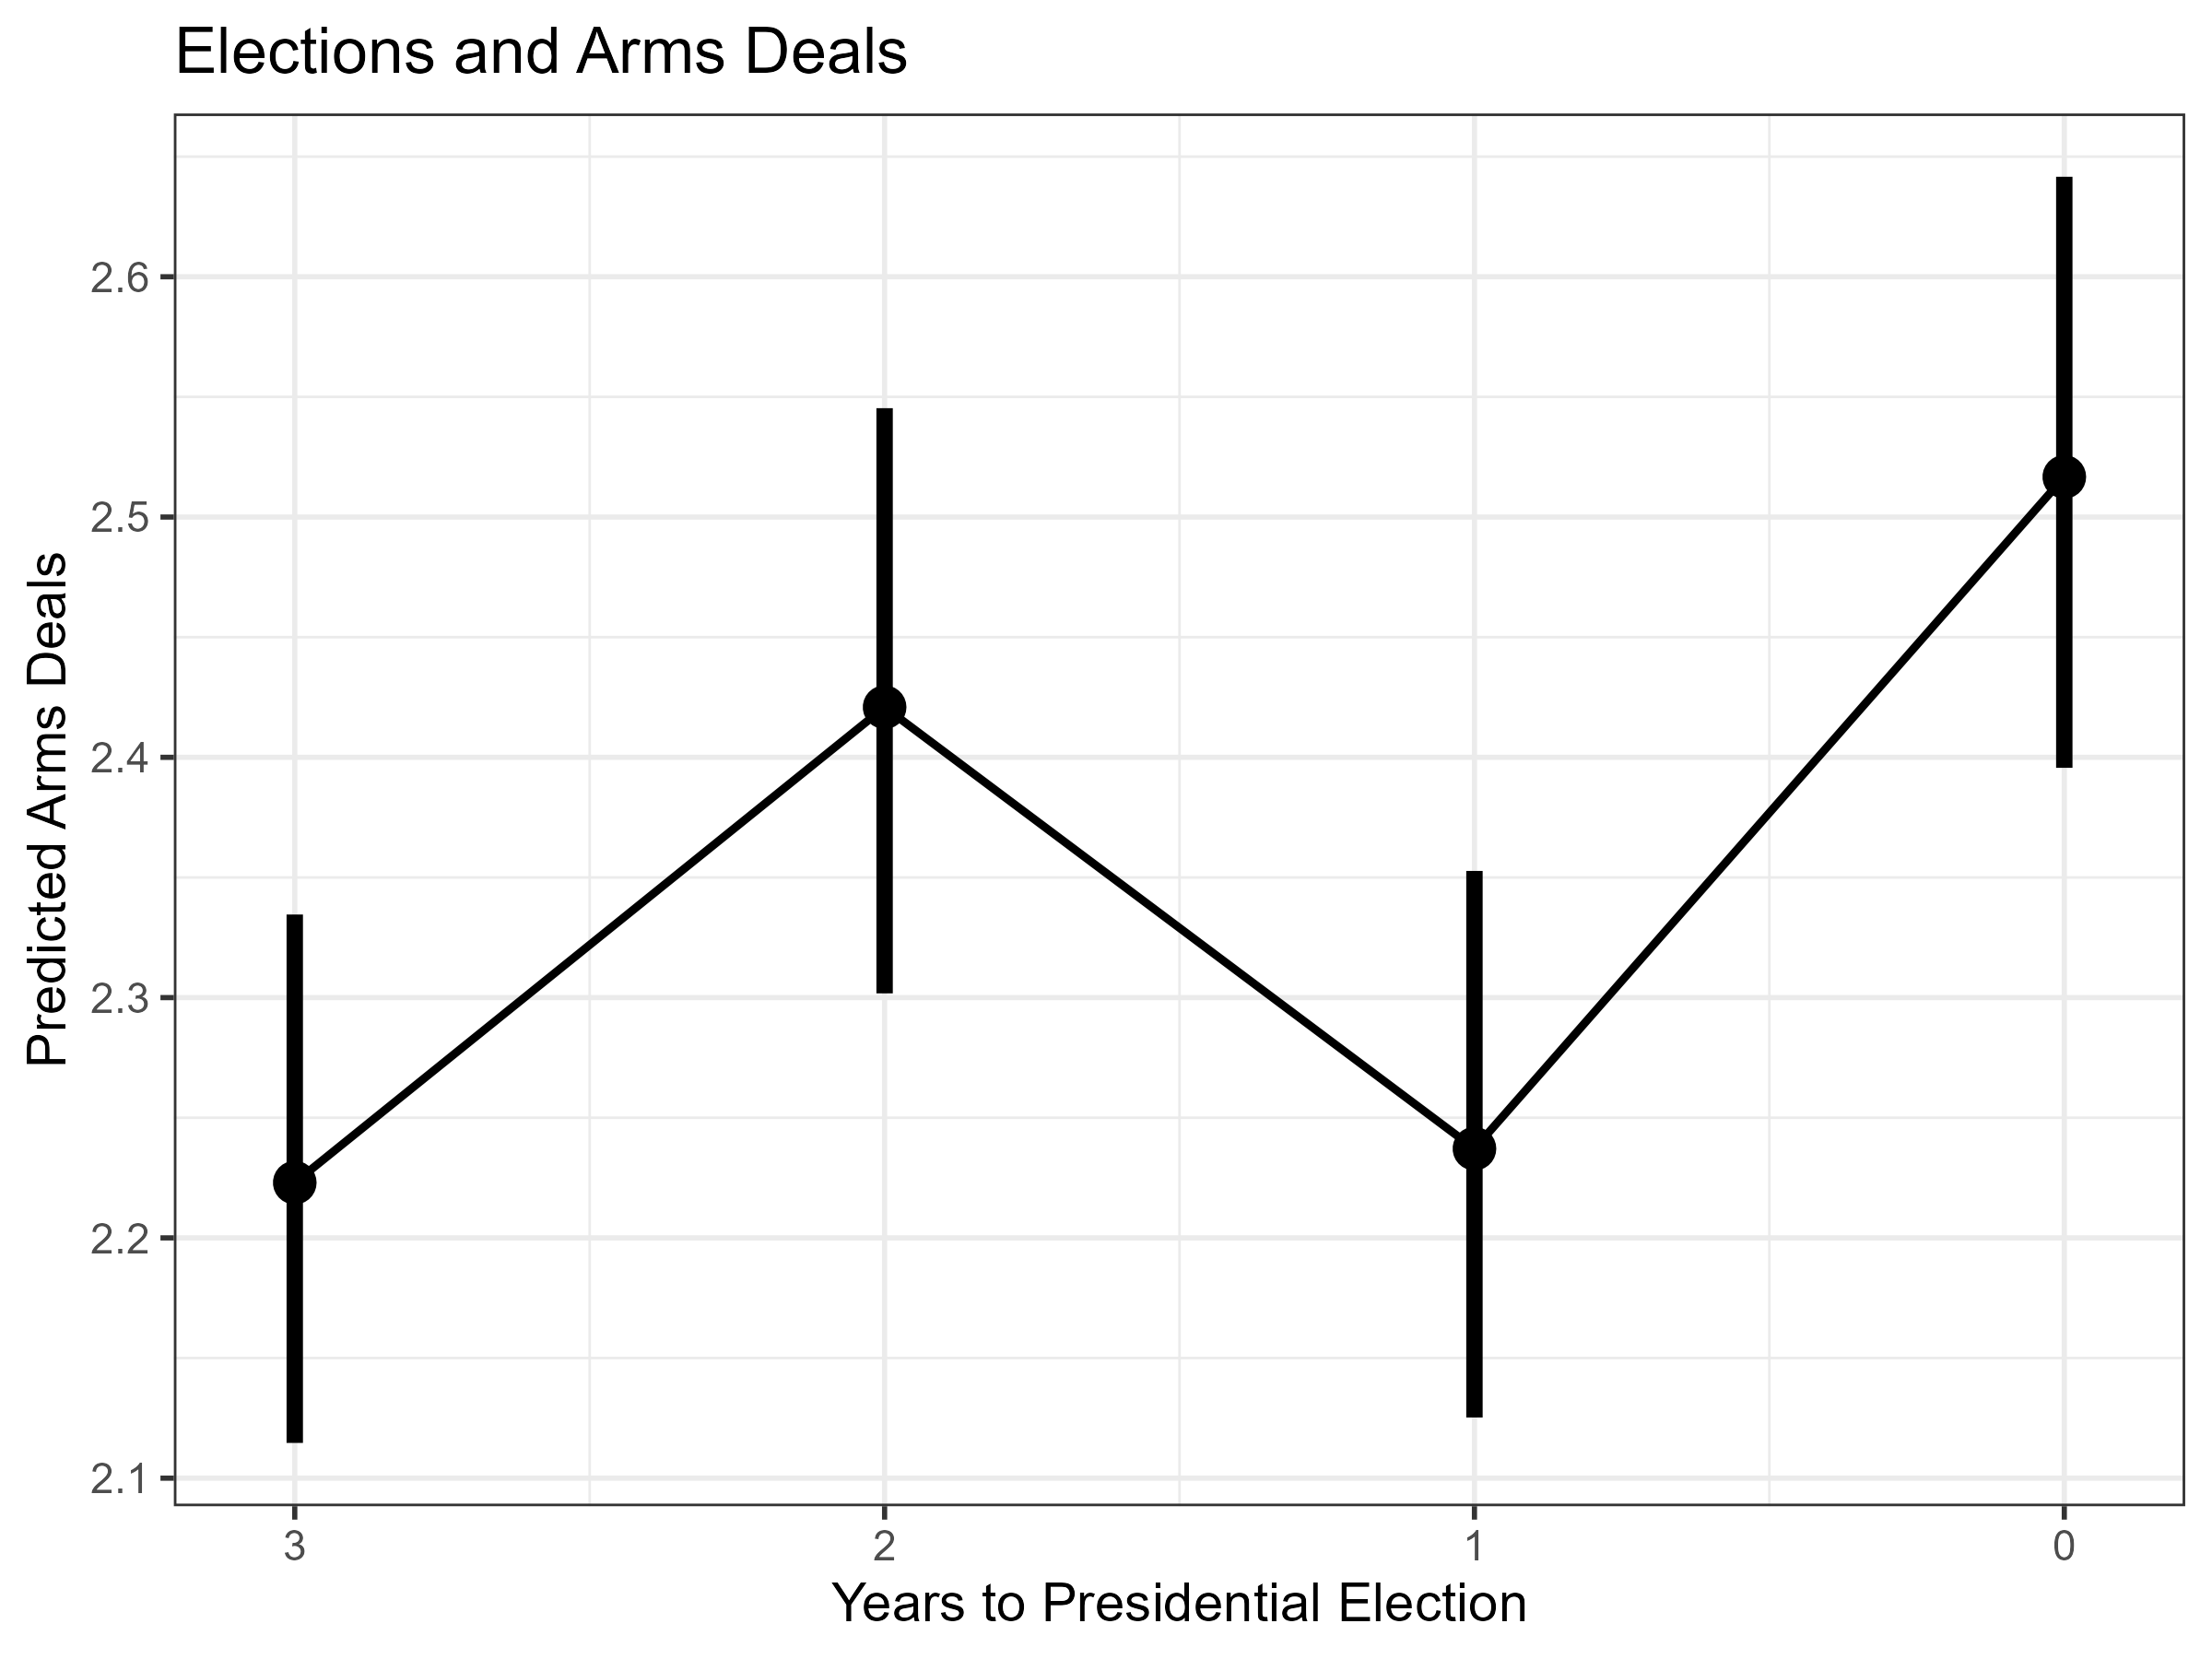
\includegraphics[width=0.95\textwidth]{elec-pred-deals.png}
	\caption{Predicted arms deals by the United States across the presidential election cycle, all else equal. Estimates from a hurdle Poisson model of arms deals between 1950 and 2014. }
	\label{fig:elec-pred-deals}
\end{figure}



\subsection{Dropping Potential Outliers}

Another possibility is that the results are due to a few outlier countries, such as Saudi Arabia. 
If one country is responsible for the overall pattern, then this argument has limited generalizability. 
To check this, I refit the hurdle poisson model of arms deals six times, dropping Saudi Arabia, the United Arab Emirates, Iran, Brazil and Argentina as potential outlier autocracies who purchased many U.S. arms. 
As \autoref{fig:democ-deals-pred-drop} shows, dropping potential outliers does not change the results. 
The presidential election year increase in deals is slightly smaller when I remove Saudi Arabia, but there is still a clear jump in arms purchases by autocracies.  


\begin{figure}[htpb]
	\centering
		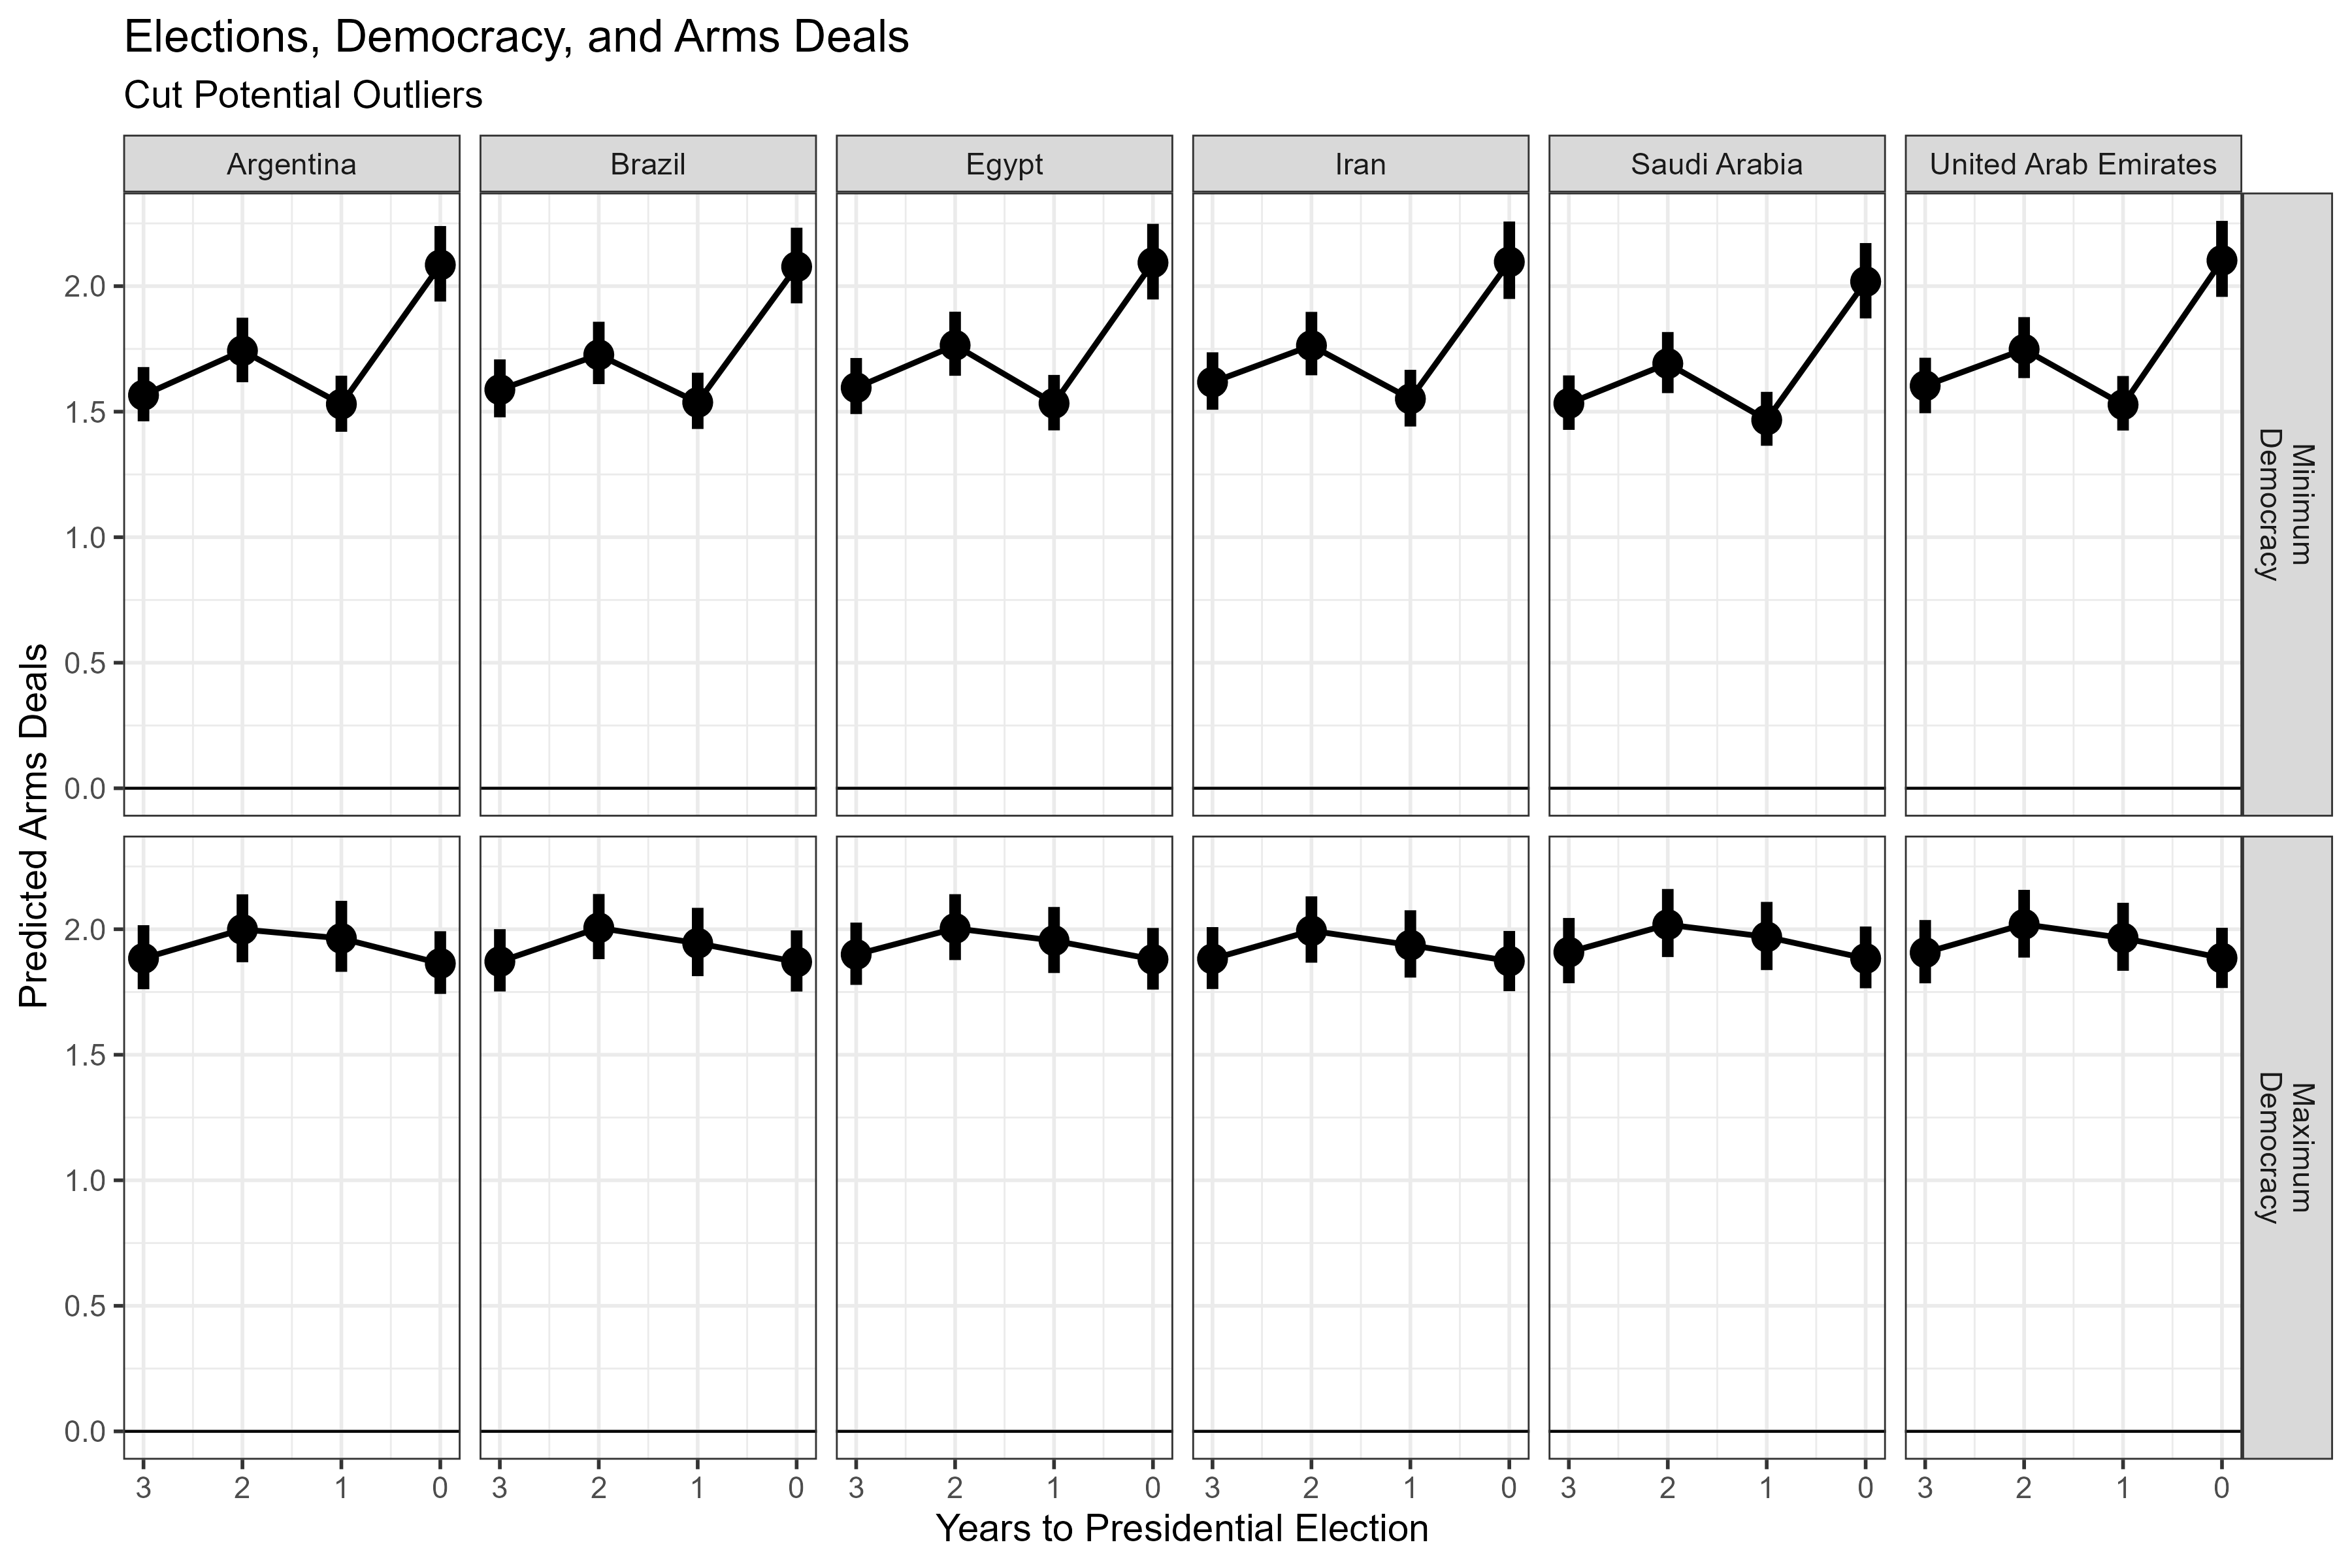
\includegraphics[width=0.95\textwidth]{democ-deals-pred-drop.png}
	\caption{Predicted arms deals by the United States across the presidential election cycle in six models, each of which drops a potential outlier arms purchaser. Estimates from a hurdle Poisson model of arms deals between 1950 and 2014. Polyarchy fixed to minimum and maximum for predictions.}
	\label{fig:democ-deals-pred-drop}
\end{figure}


\subsection{Linear Estimate of Time to Election}

In the manuscript, I use dummy variables marking years to a presidential election to capture election proximity. 
As I show here, using one measure of years to an election gives similar inferences. 
The downside is that it smooths over the fall in autocratic deals in years between Congressional and Presidential elections, as \autoref{fig:democ-deals-pred-lin} makes clear. 


\begin{figure}[htpb]
	\centering
		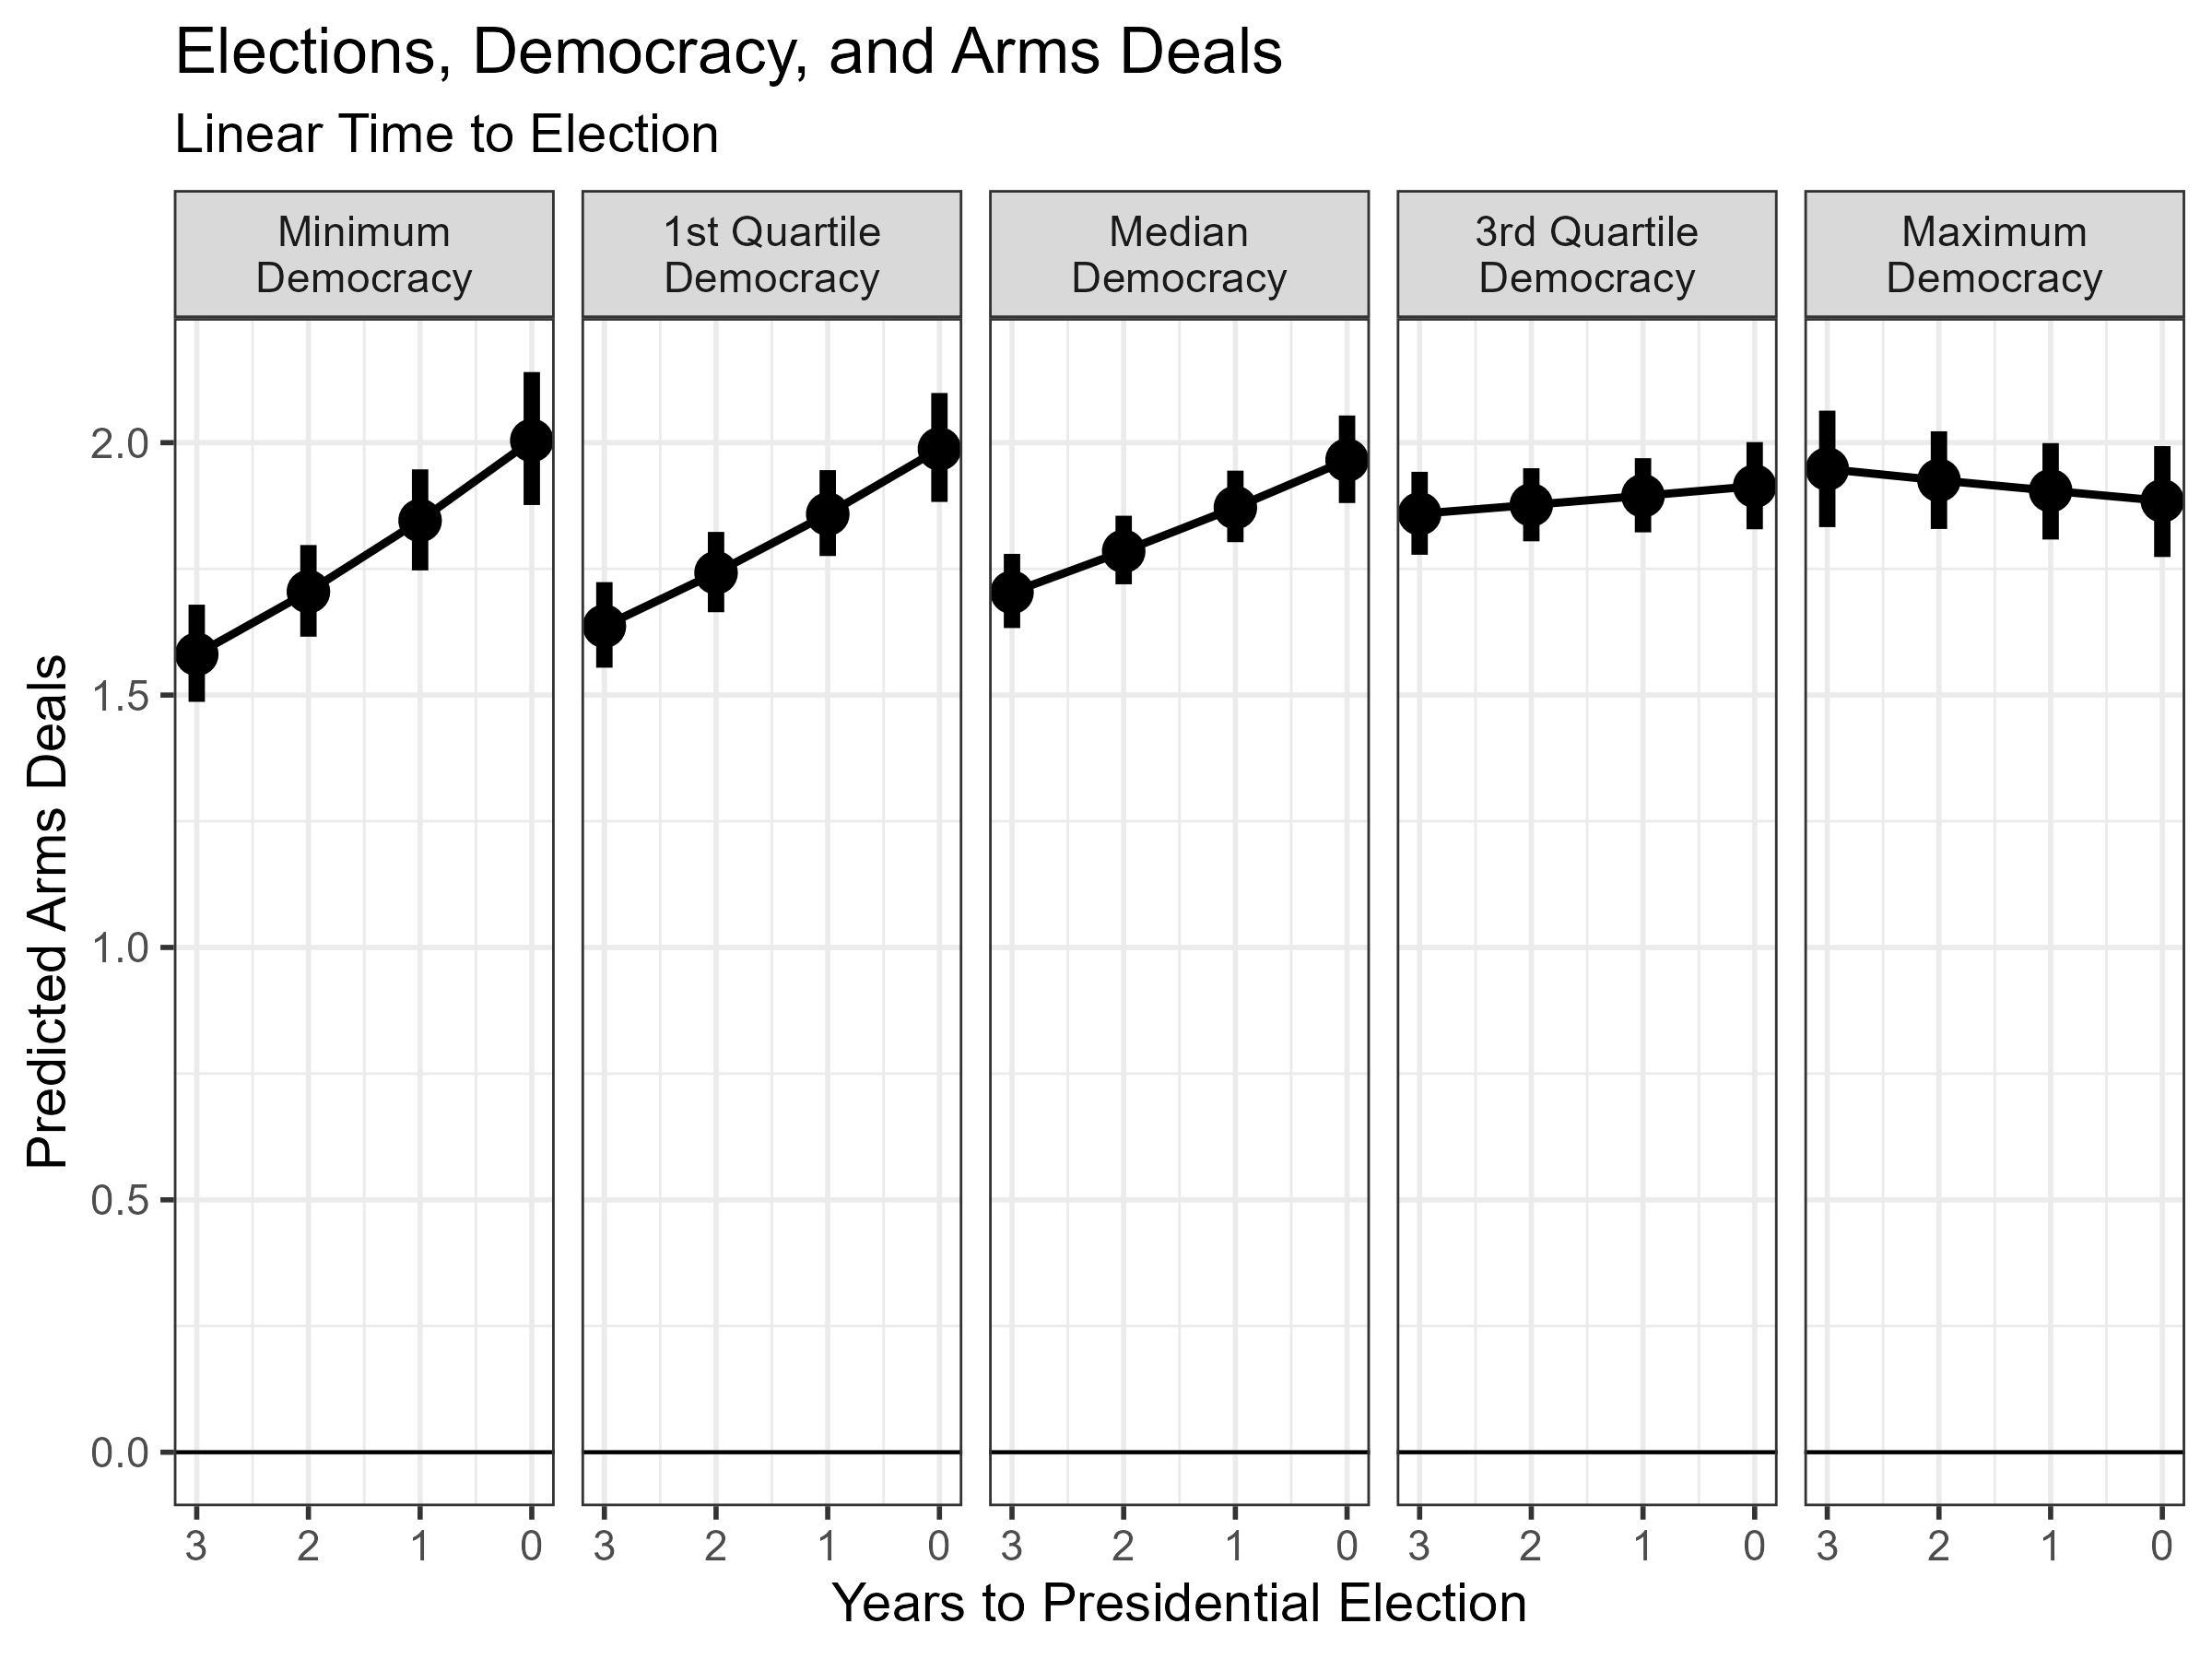
\includegraphics[width=0.95\textwidth]{democ-deals-pred-lin.png}
	\caption{Predicted arms deals by the United States across the presidential election cycle in six models, each of which drops a potential outlier arms purchaser. Estimates from a hurdle Poisson model of arms deals between 1950 and 2014. Polyarchy fixed to minimum and maximum for predictions.}
	\label{fig:democ-deals-pred-lin}
\end{figure}

\subsection{Alternative Estimators}


The same pattern is also apparent if I use three alternative models of arms deals, election timing and autocracy. 
While the hurdle Poisson is the most theoretically appropriate specification, standard Poisson and zero-inflated Poisson models give similar inferences.
The Poisson results hold without controls as well.
I plot predicted arms deals across recipient democracy and election timing from each of these models in \autoref{fig:deals-pred-nocont}, \autoref{fig:deals-pred-pois} and \autoref{fig:deals-pred-zip}. 
All three estimators suggest increasing arms deals for autocratic allies as elections approach, and little change in deals with democratic allies near presidential elections. 


\begin{figure}[htpb]
	\centering
		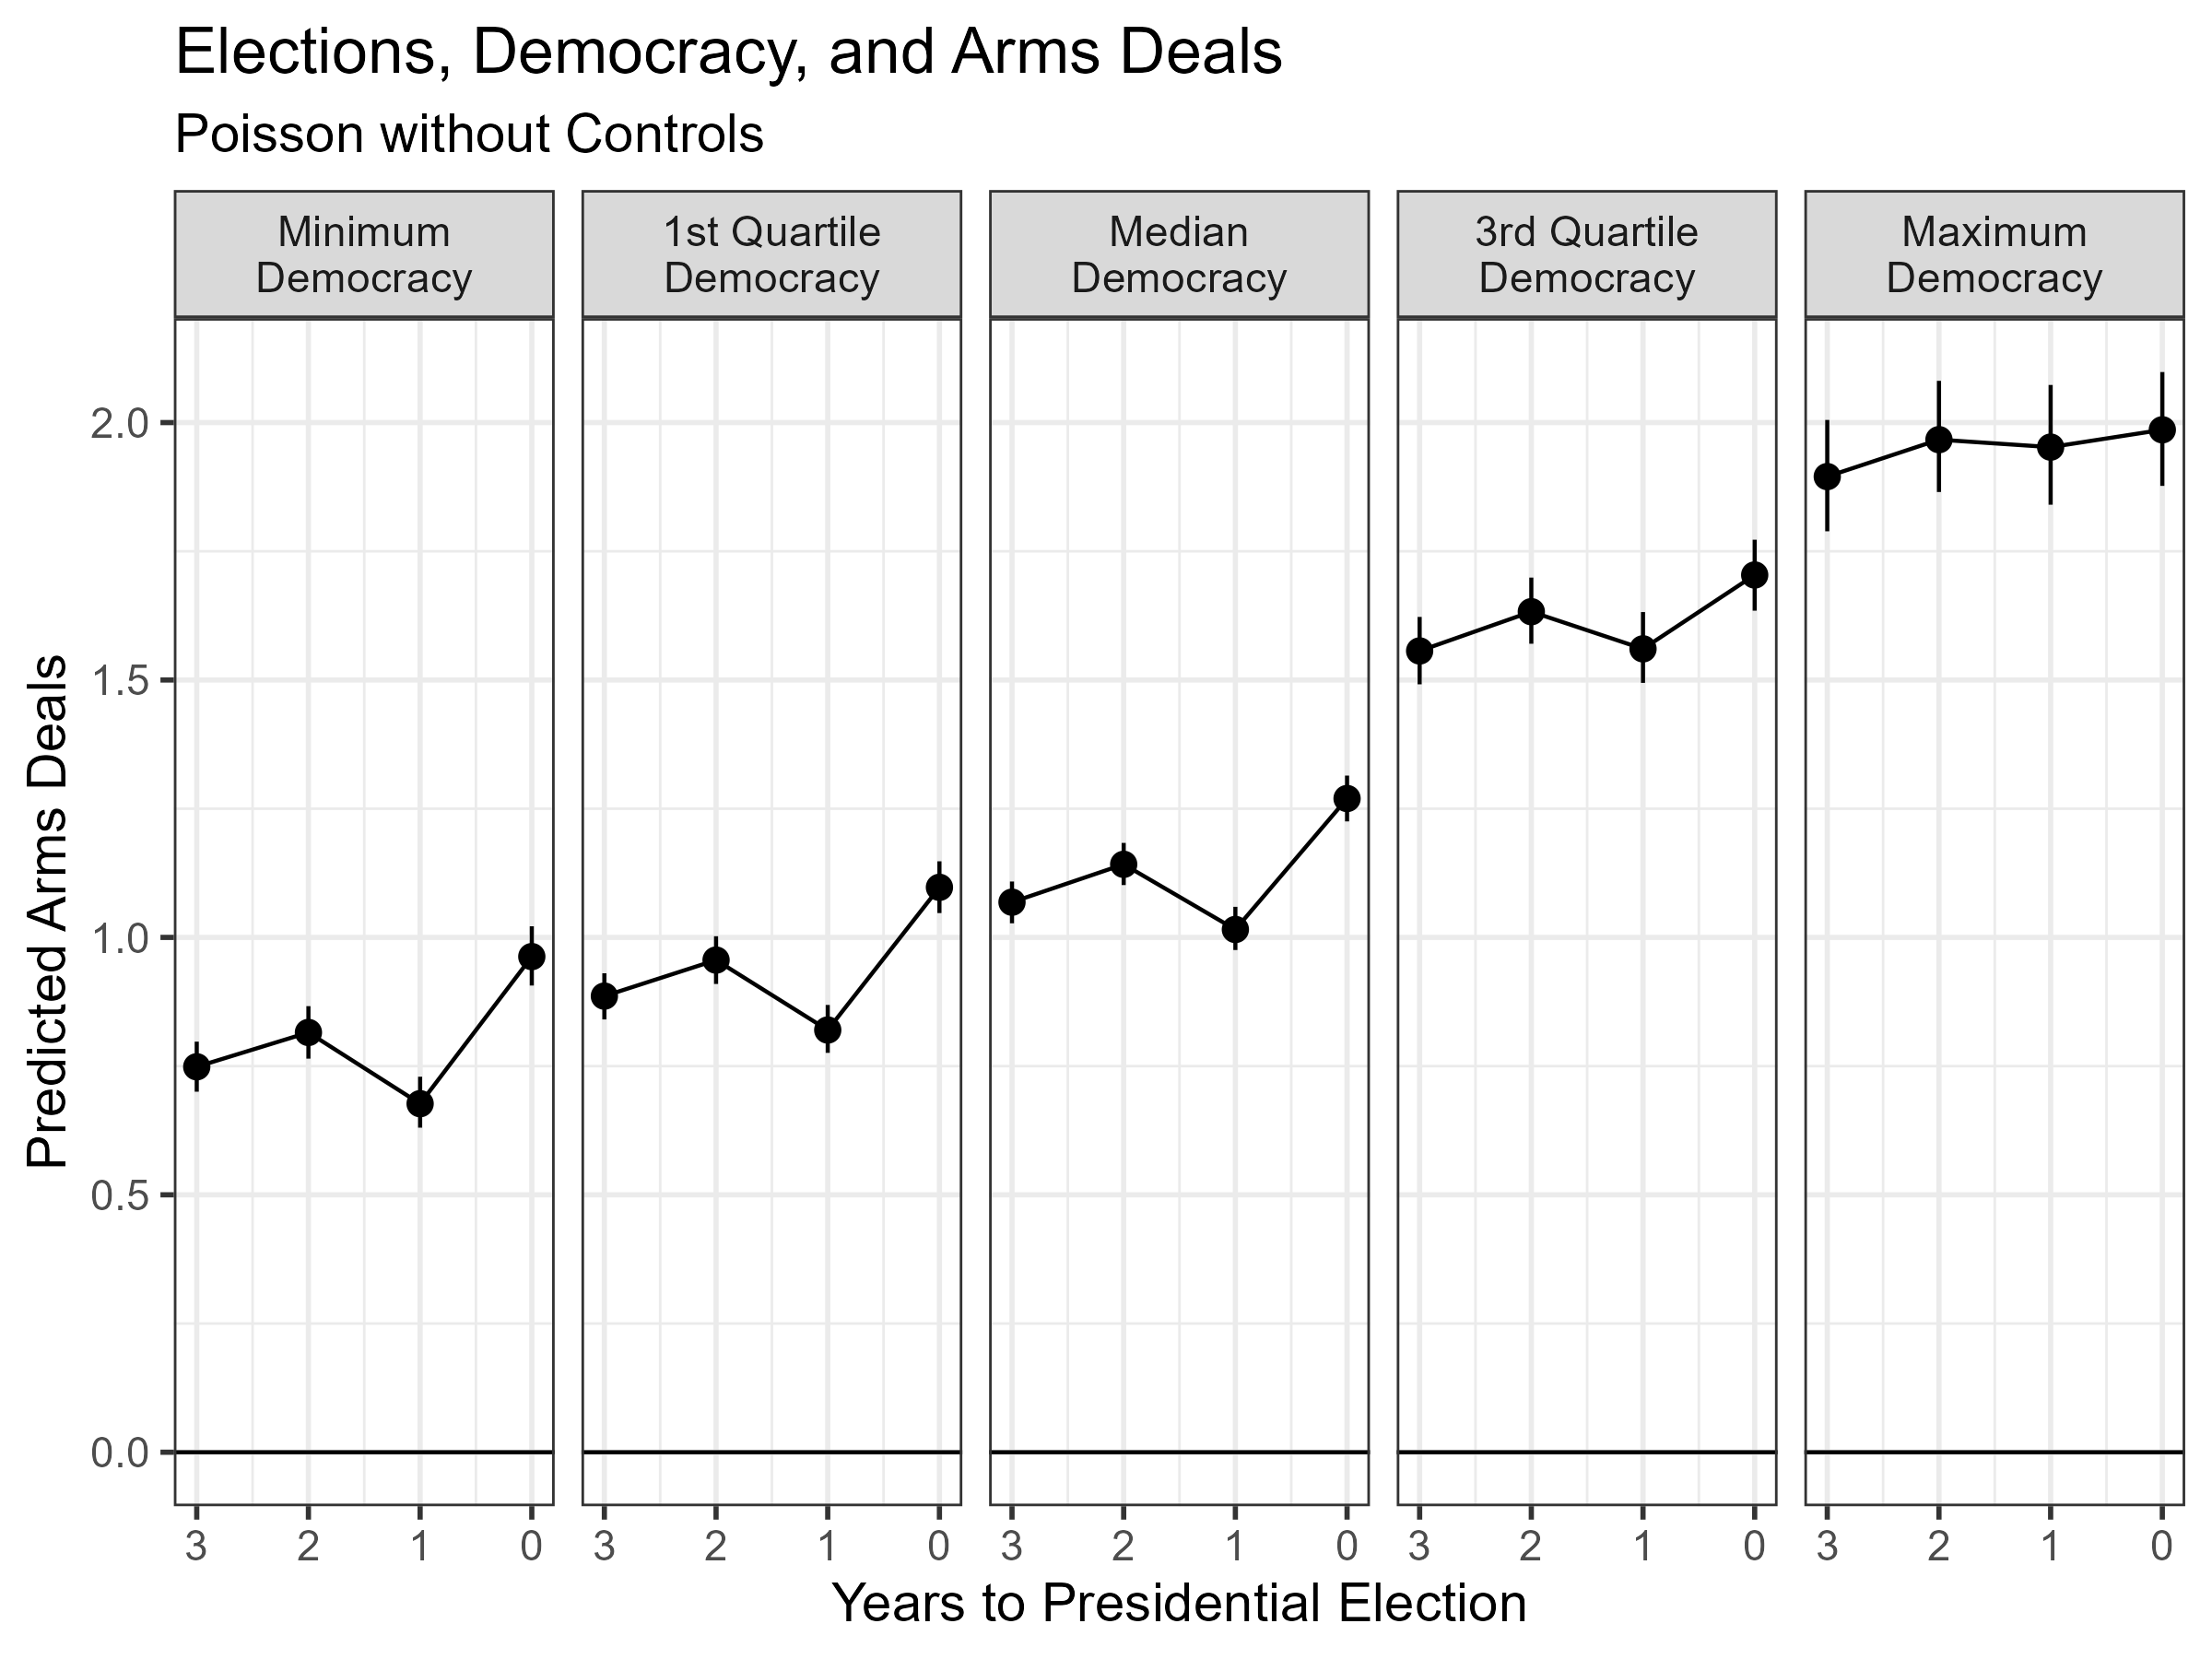
\includegraphics[width=0.95\textwidth]{nocont-deals-pred.png}
	\caption{Predicted arms deals between the United States and other states 1950 to 2014 by presidential election proximity and partner democracy based on a Poisson regression model with only those two variables and no controls. Points mark the estimates and error bars summarize the 90\% credible interval.}
	\label{fig:deals-pred-nocont}
\end{figure}



\begin{figure}[htpb]
	\centering
		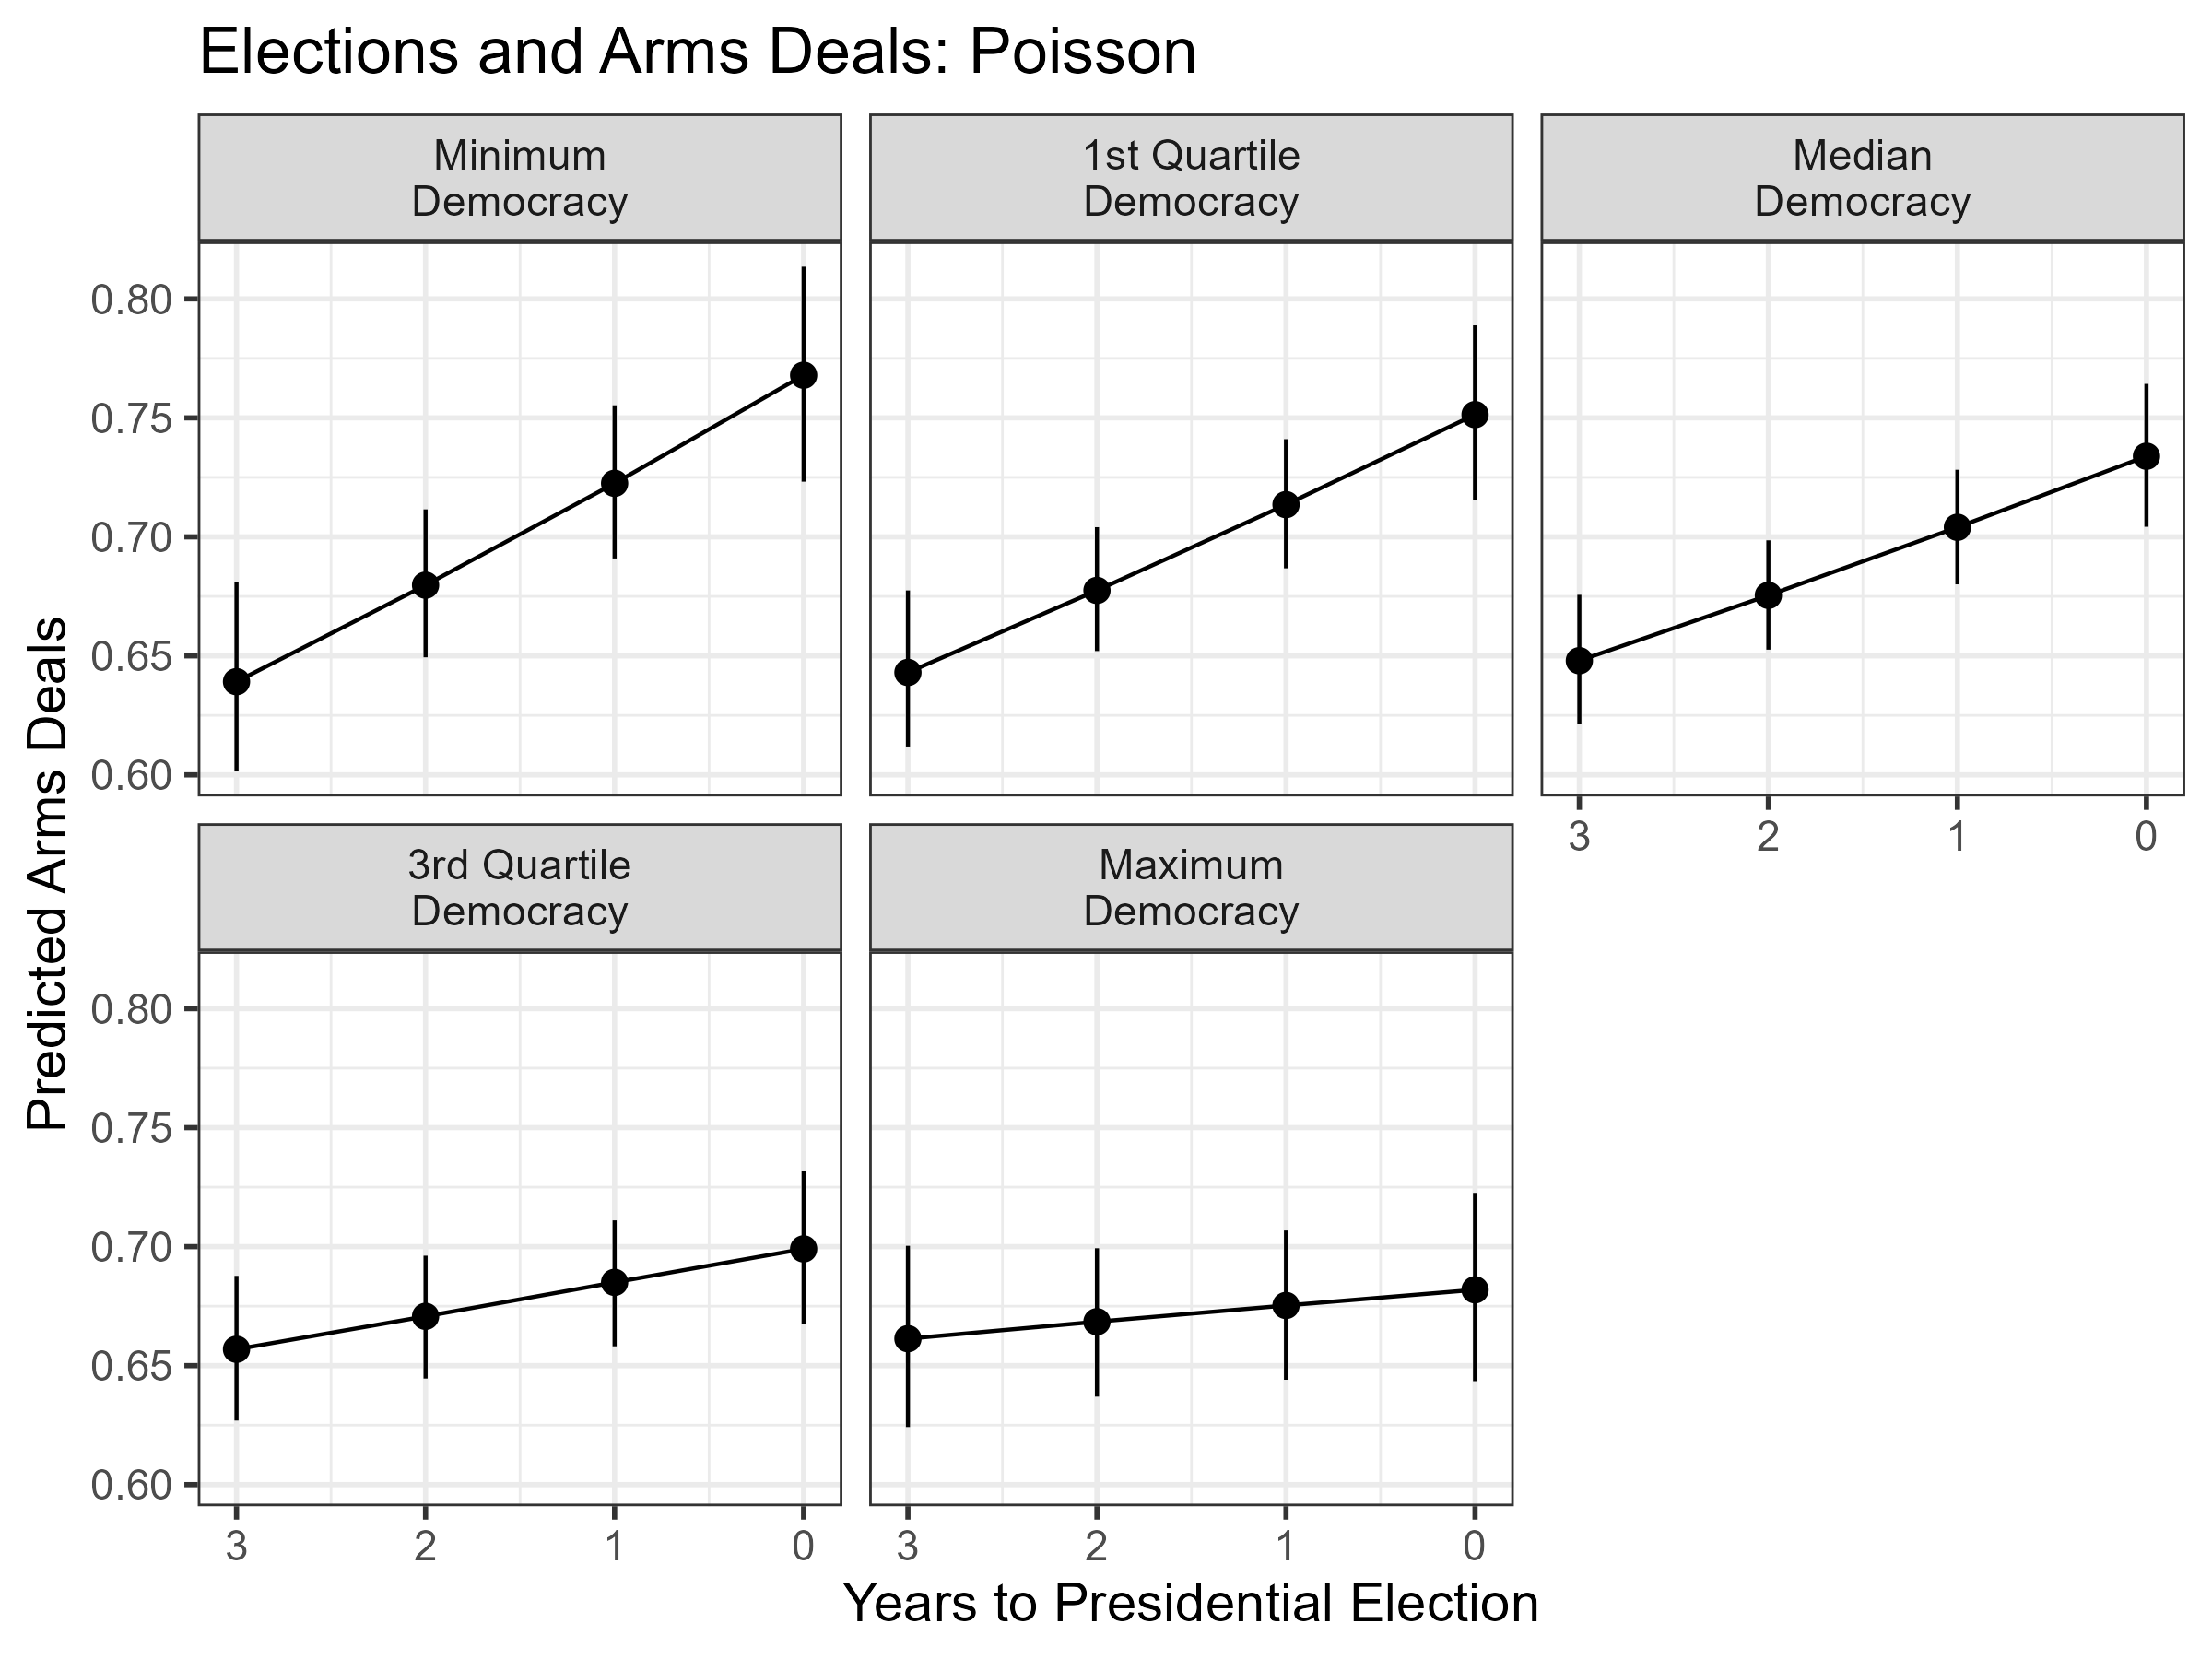
\includegraphics[width=0.95\textwidth]{deals-pred-pois.png}
	\caption{Predicted arms deals between the United States and other states 1950 to 2014 by presidential election proximity and partner democracy based on a Poisson model. Points mark the estimates and error bars summarize the 90\% credible interval.}
	\label{fig:deals-pred-pois}
\end{figure}



\begin{figure}[htpb]
	\centering
		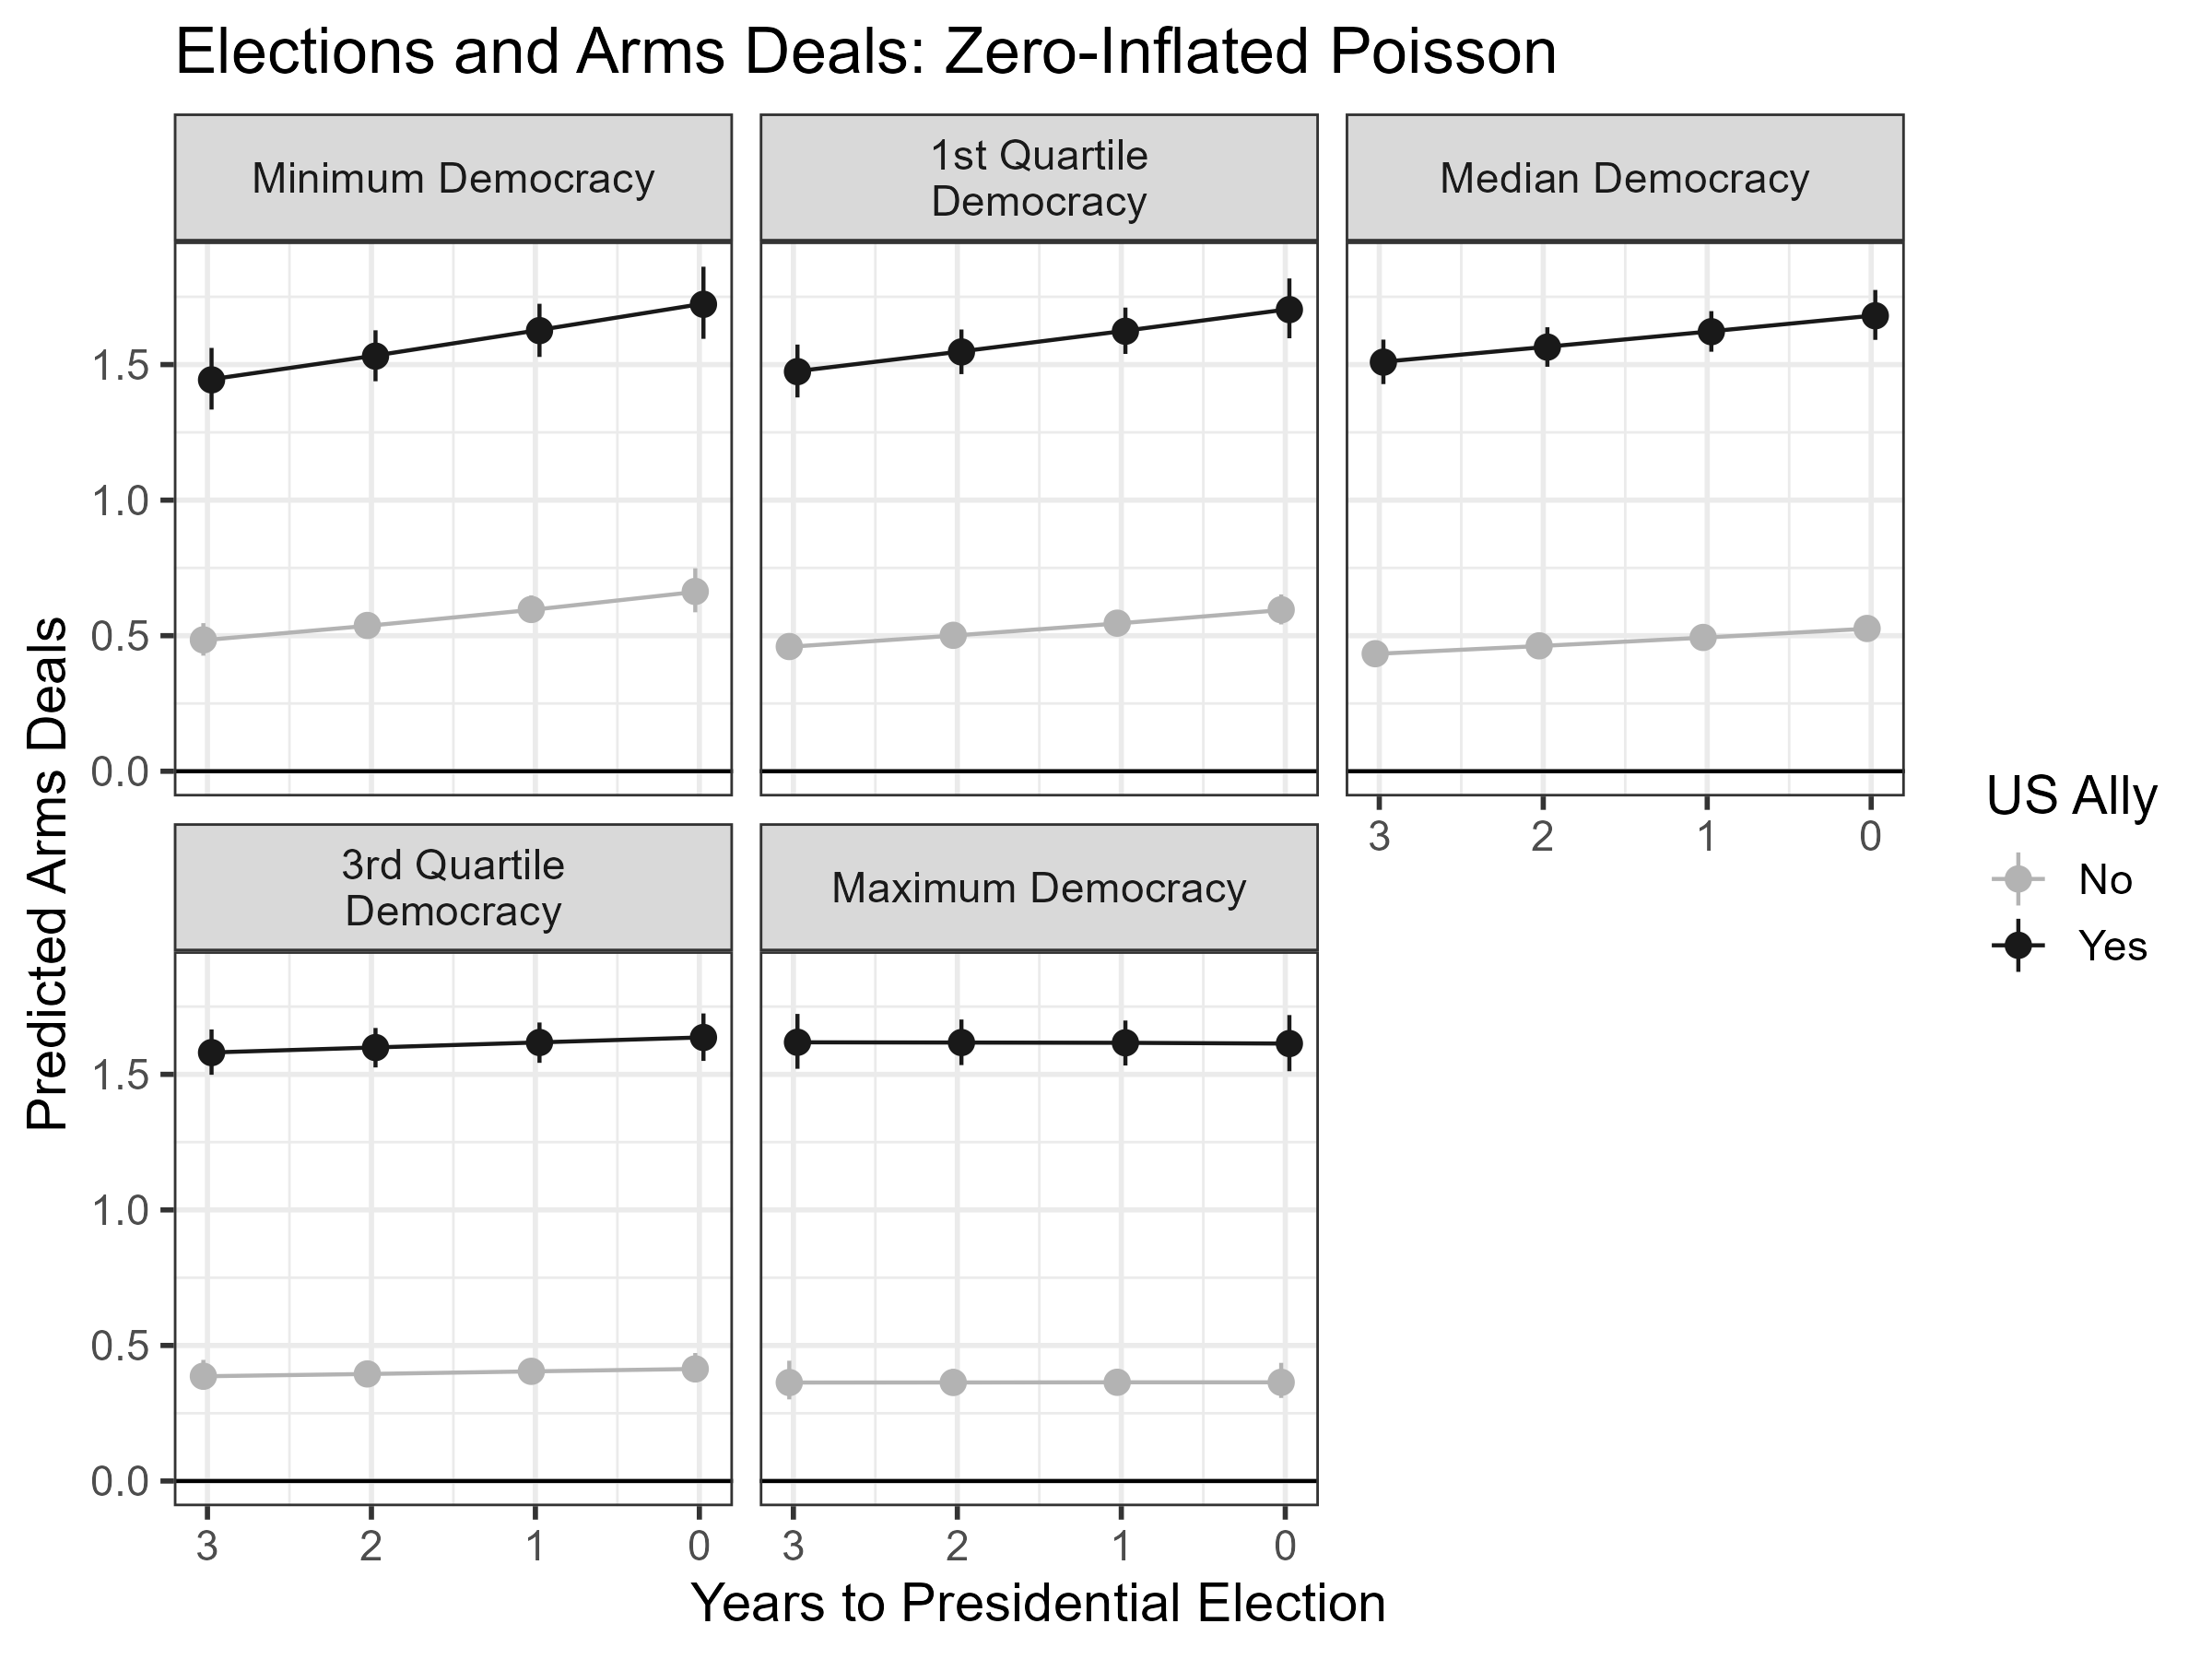
\includegraphics[width=0.95\textwidth]{deals-pred-zip.png}
	\caption{{Predicted arms deals between the United States and other states 1950 to 2014 by presidential election proximity and partner democracy based on a zero-inflated Poisson model. Points mark the estimates and error bars summarize the 90\% credible interval.}}
	\label{fig:deals-pred-zip}
\end{figure}

\newpage

\subsection{Posterior Predictive Checks}


This final check shows the predictive performance of the hurdle Poisson model, relative to a Poisson and negative binomial specification. 
While no model perfectly captures the lumpy outcome distribution, the hurdle Poisson is much better 
First, I show the posterior predictive check for the hurdle Poisson in \autoref{fig:pp-check-deals}. 


\autoref{fig:pp-check-deals}, \autoref{fig:pois-pp-check} and \autoref{fig:nb-pp-check} are rootograms, which plot expected counts against observed counts. 
In both figures, the line gives the expected counts based on the model, and the bars mark observed counts. 
Bars that exceed zero are counts the model under predicts, while bars above zero show underpredicted values. 
As a result, the hurdle Poisson predicts zero values well, underpredicts some large values, and overpredicts a few small values. 



\begin{figure}[htpb]
	\centering
		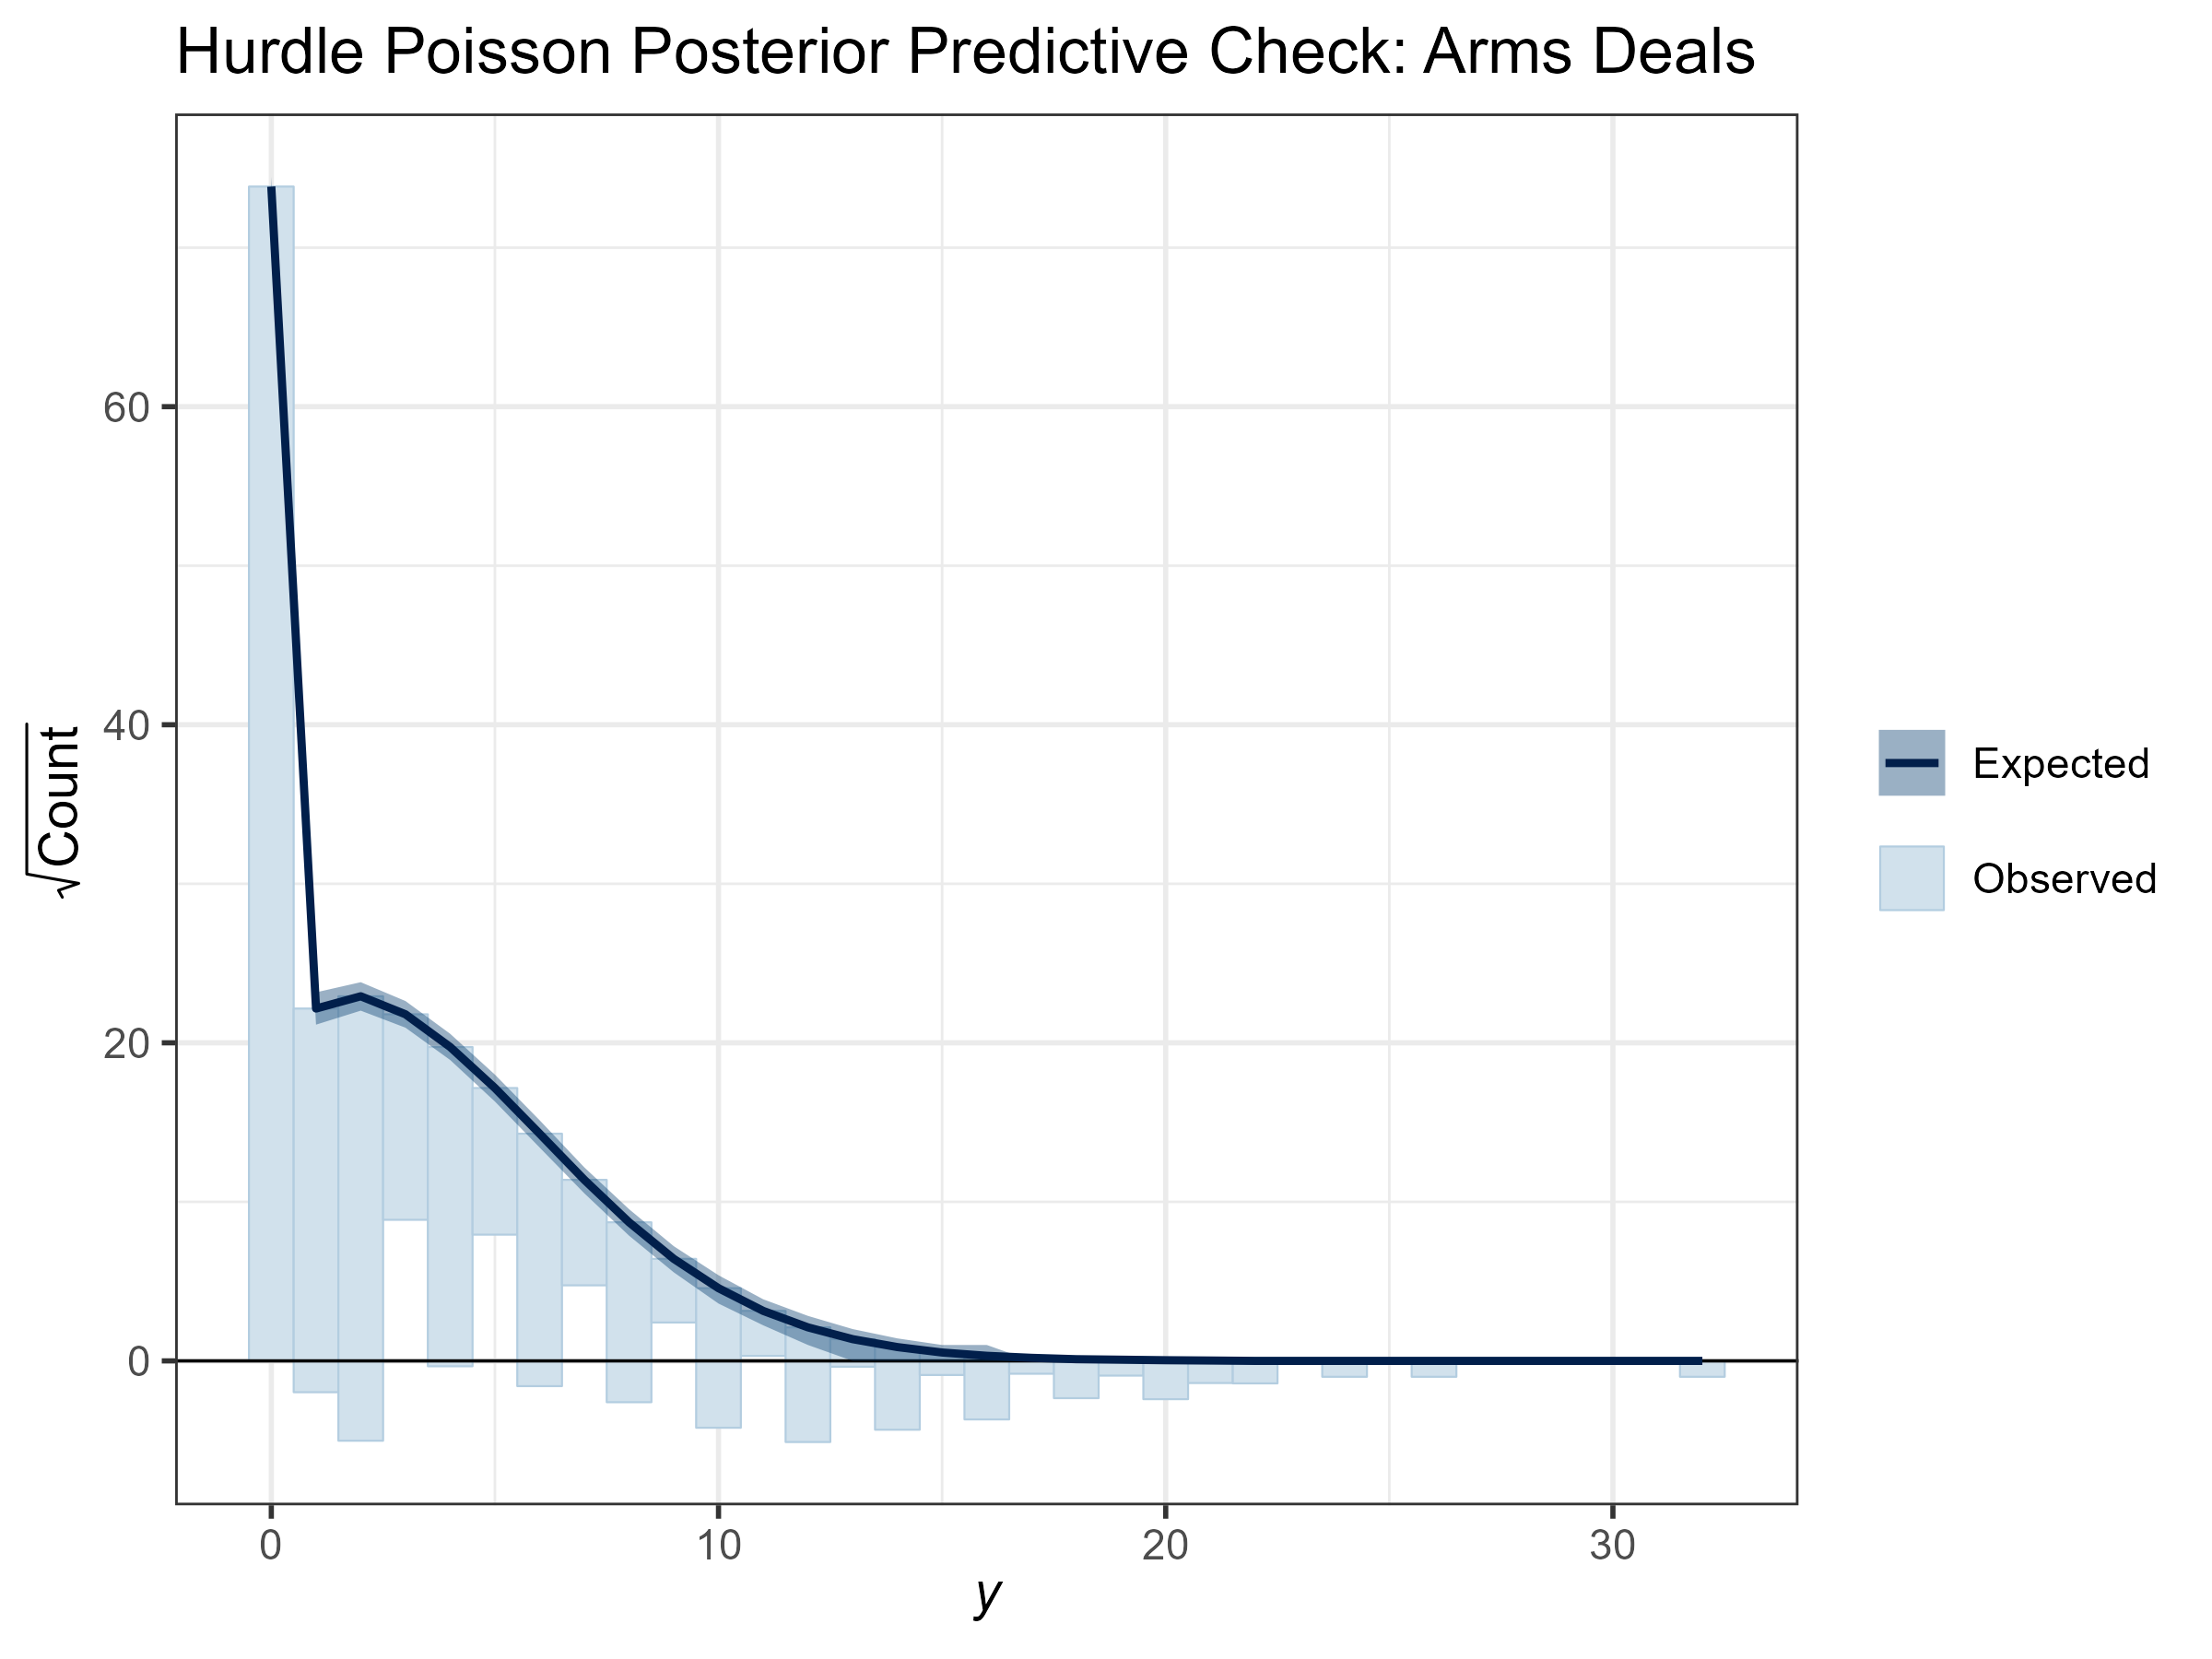
\includegraphics[width=0.95\textwidth]{pp-check-deals.png}
	\caption{Posterior predictive check of the hurdle Poisson model of U.S. arms deals. The fitted line gives the expected counts and bars show the observed distribution.}
	\label{fig:pp-check-deals}
\end{figure}


Relative to the hurdle, a regular Poisson model under-predicts zeros, as \autoref{fig:pois-pp-check} demonstrates. 
This also reduces predictive accuracy for non-zero deals. 


\begin{figure}[htpb]
	\centering
		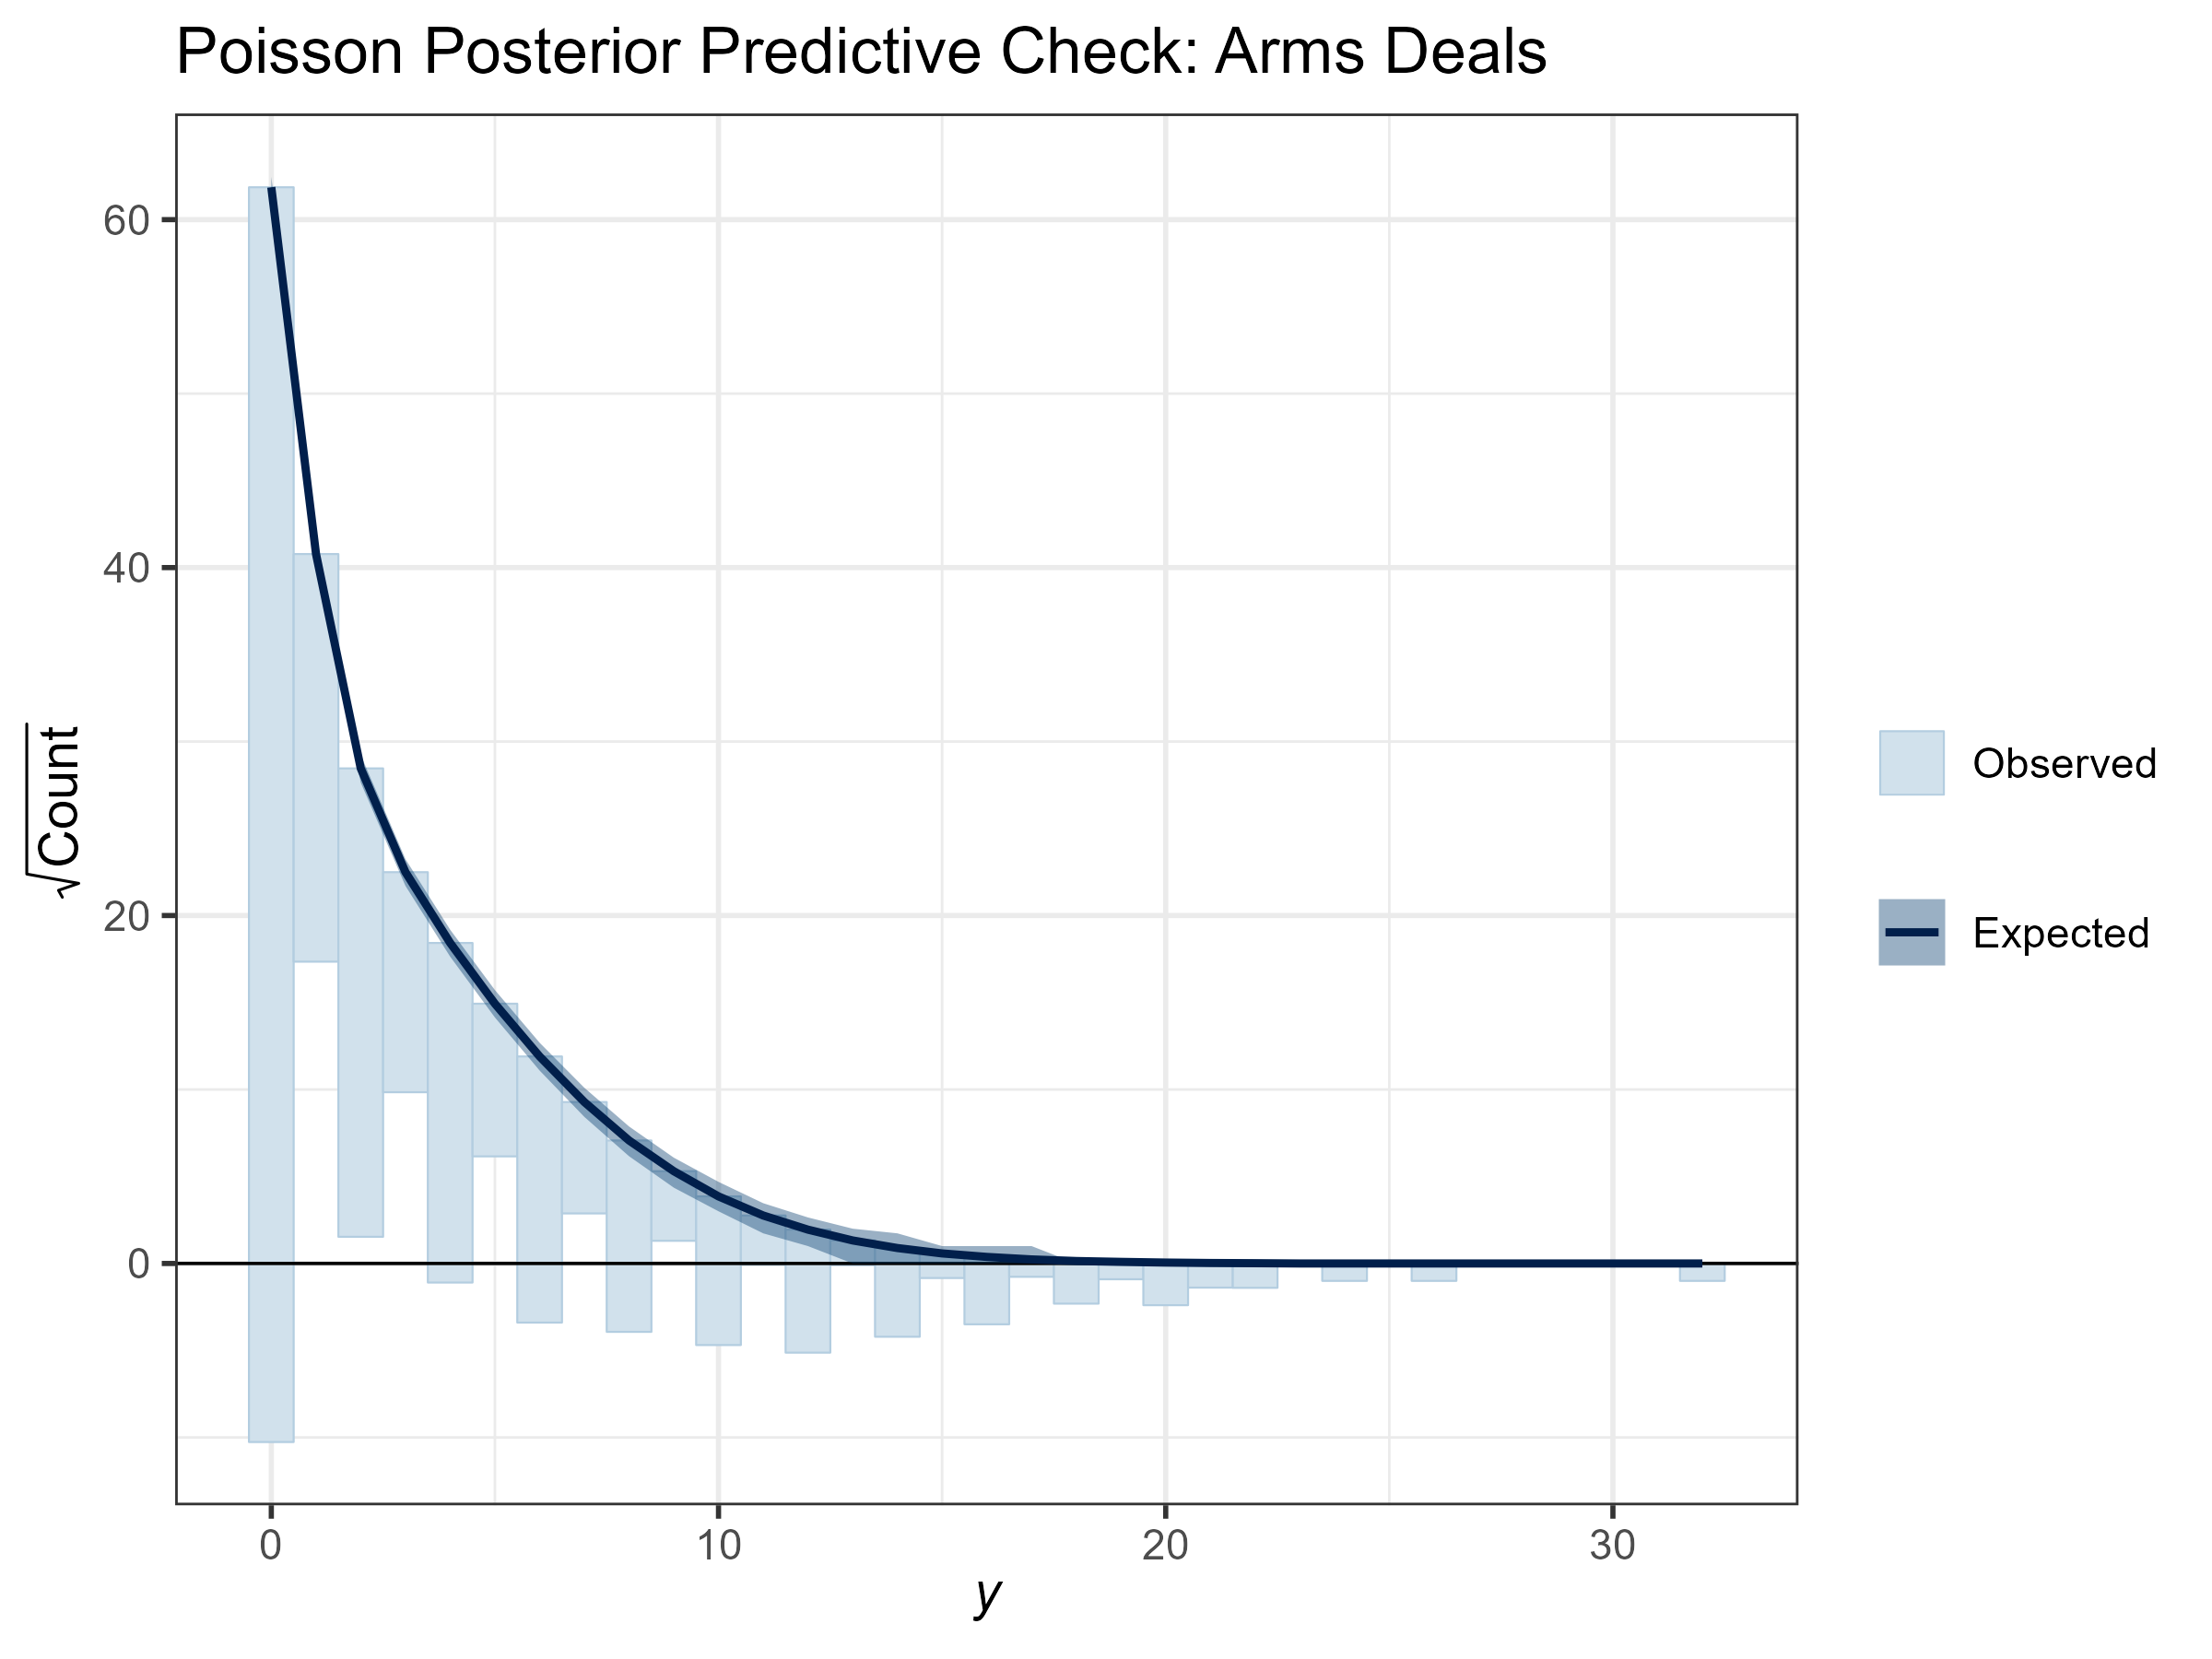
\includegraphics[width=0.95\textwidth]{pois-pp-check.png}
	\caption{Posterior predictive check of a Poisson model of U.S. arms deals. The fitted line gives the expected counts and bars show the observed distribution.}
	\label{fig:pois-pp-check}
\end{figure}


While the lumpy distribution of deals complicates predictions with a Poisson likelihood, a negative binomial likelihood fits poorly. 
As \autoref{fig:nb-pp-check} demonstrates, the extra variance in a negative binomial results in underpredicting almost all observed values, as well as predictions that are far above the range of the observed data. 
I therefore rely on models with a Poisson likelihood. 


\begin{figure}[htpb]
	\centering
		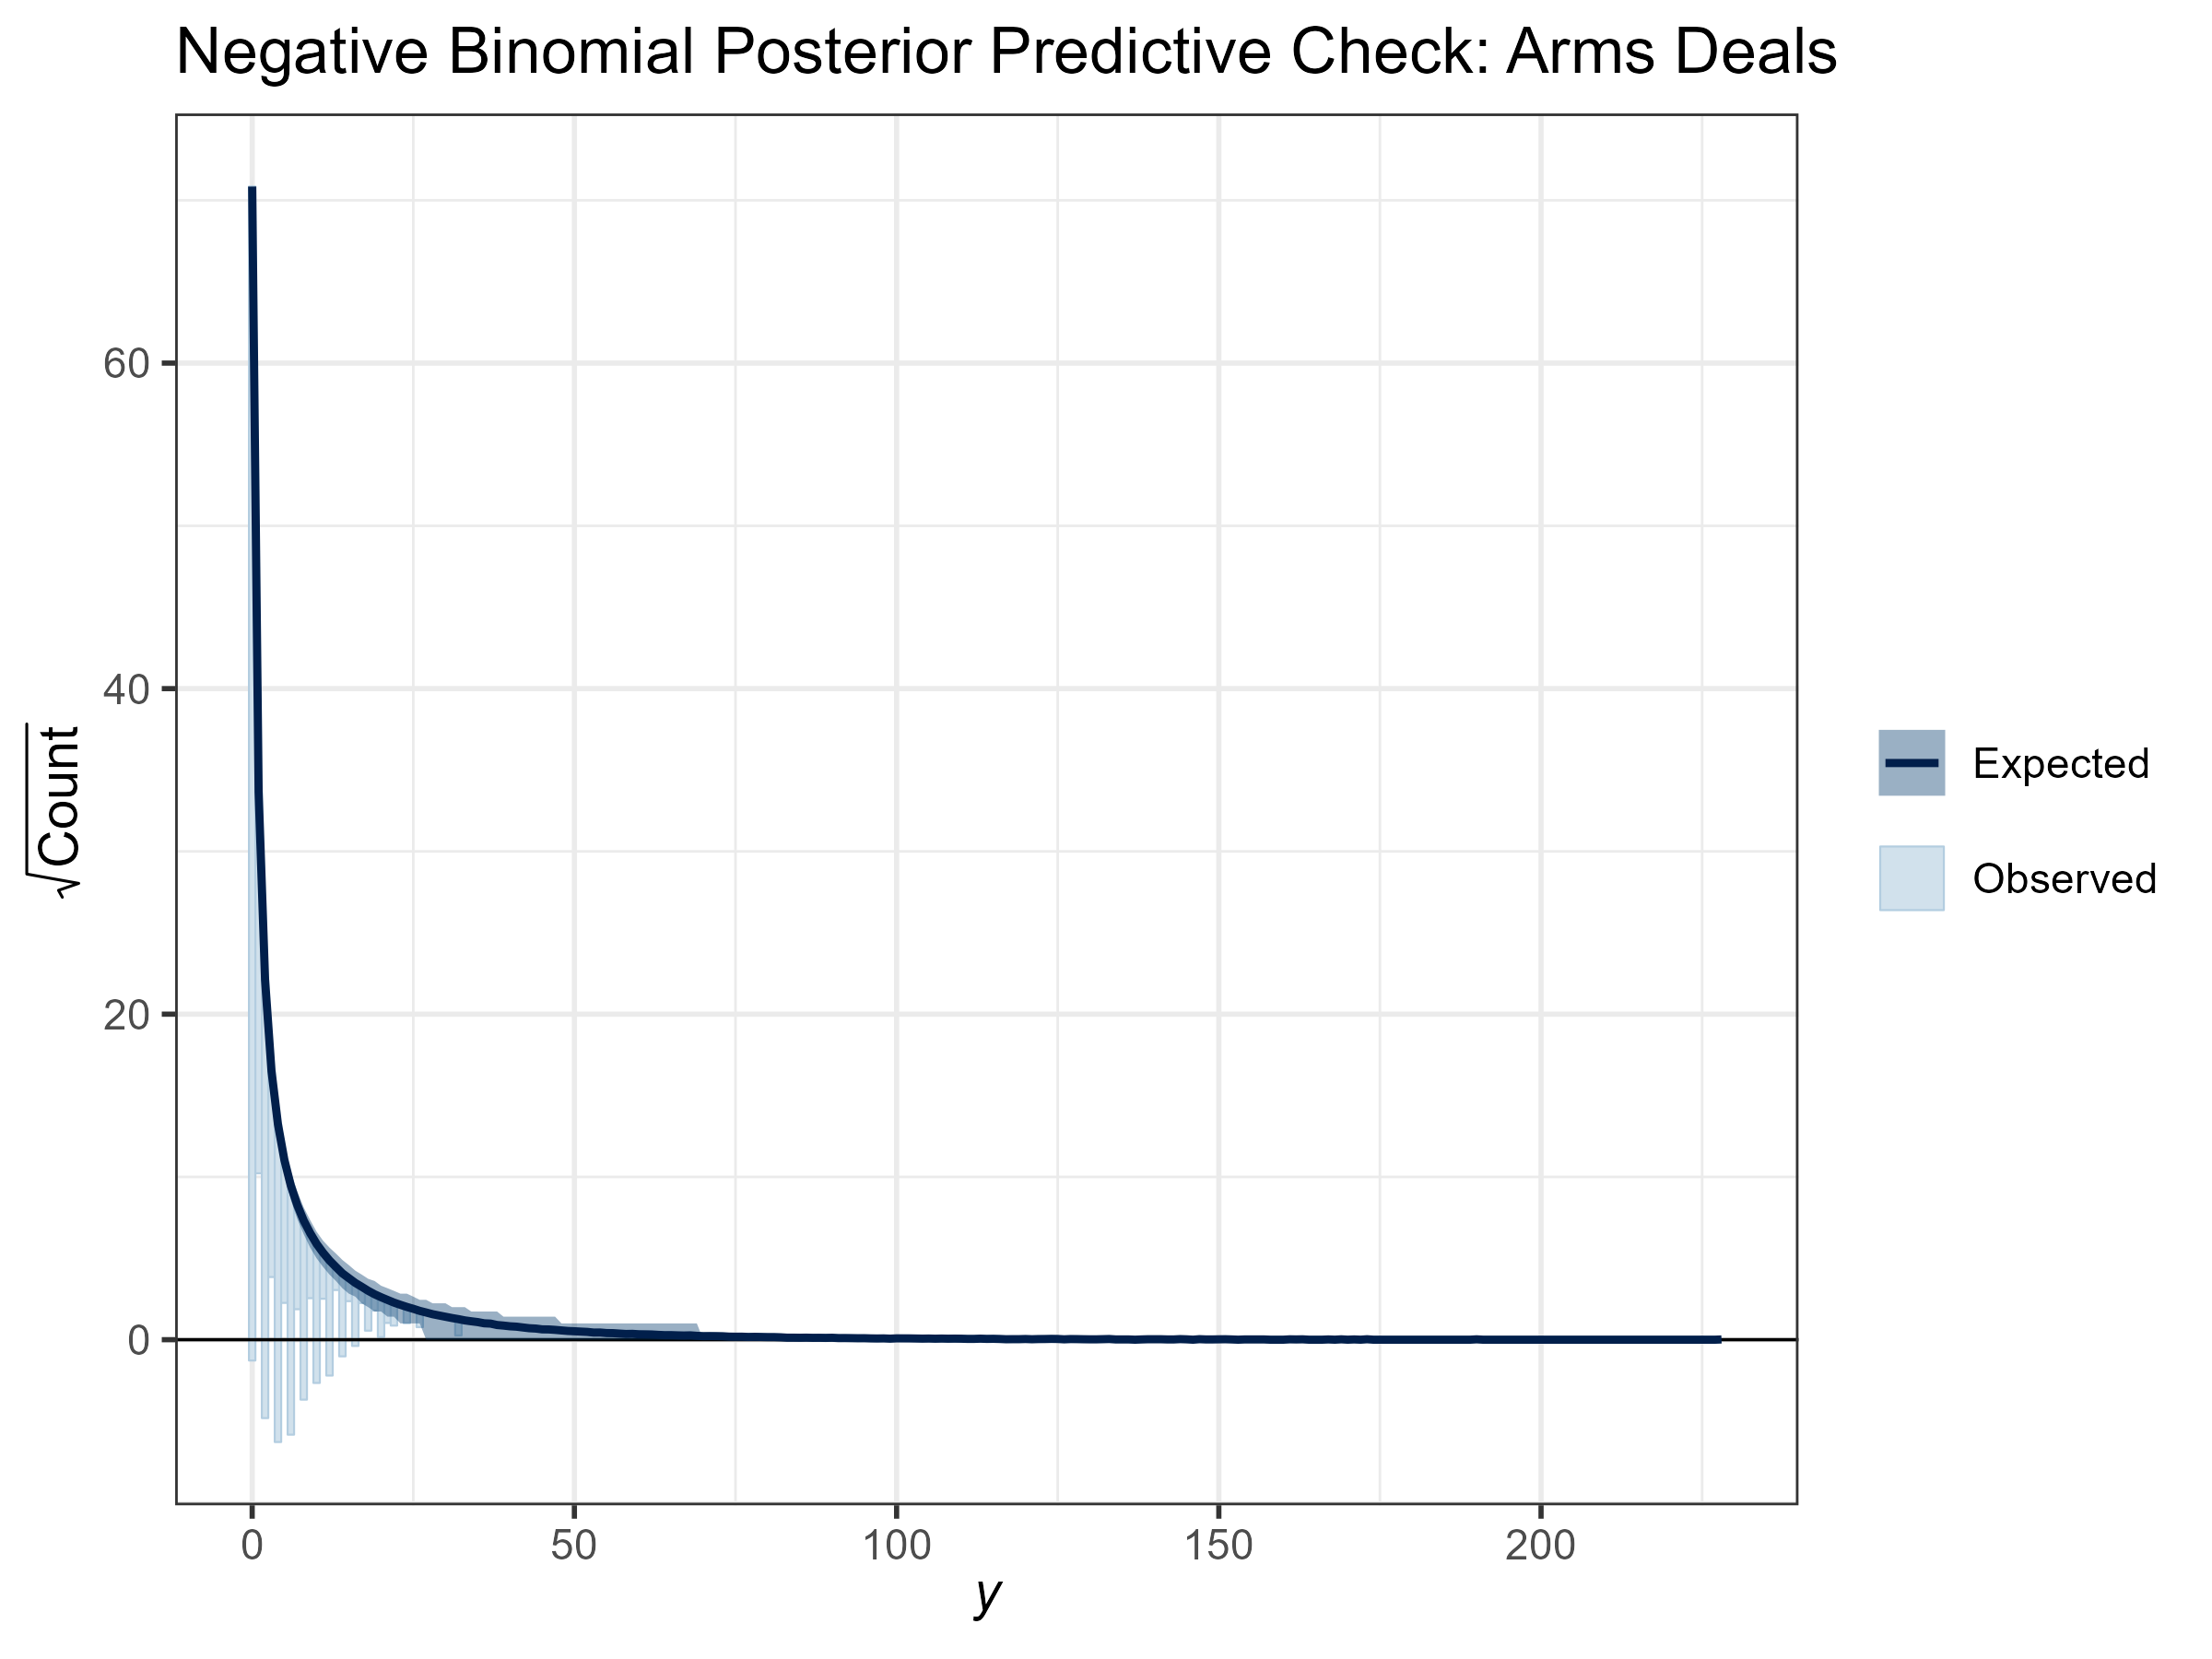
\includegraphics[width=0.95\textwidth]{nb-pp-check.png}
	\caption{Posterior predictive check of a negative binomial model of U.S. arms deals. The fitted line gives the expected counts and bars show the observed distribution.}
	\label{fig:nb-pp-check}
\end{figure}

%\newpage

\section{Contracts Model Checks} 

This section checks the second analysis, which examines the interaction between arms deals and contract awards in the 50 U.S. states. 
First, I present some raw data. 
After that, I present additional estimates from the ordered beta regression- the state varying intercepts and lagged dependent variables. 
I then show that student-t and hurdle log-normal models of defense contract changes and levels also suggest that arms deals increase contract awards to swing states. 

\subsection{Raw Contracts: Swing and Other States}

\autoref{fig:cont-swing-raw} shows that median contract awards to swing states rise as elections approach, while median awards to other states rise by much less. 

\begin{figure}[htpb]
	\centering
		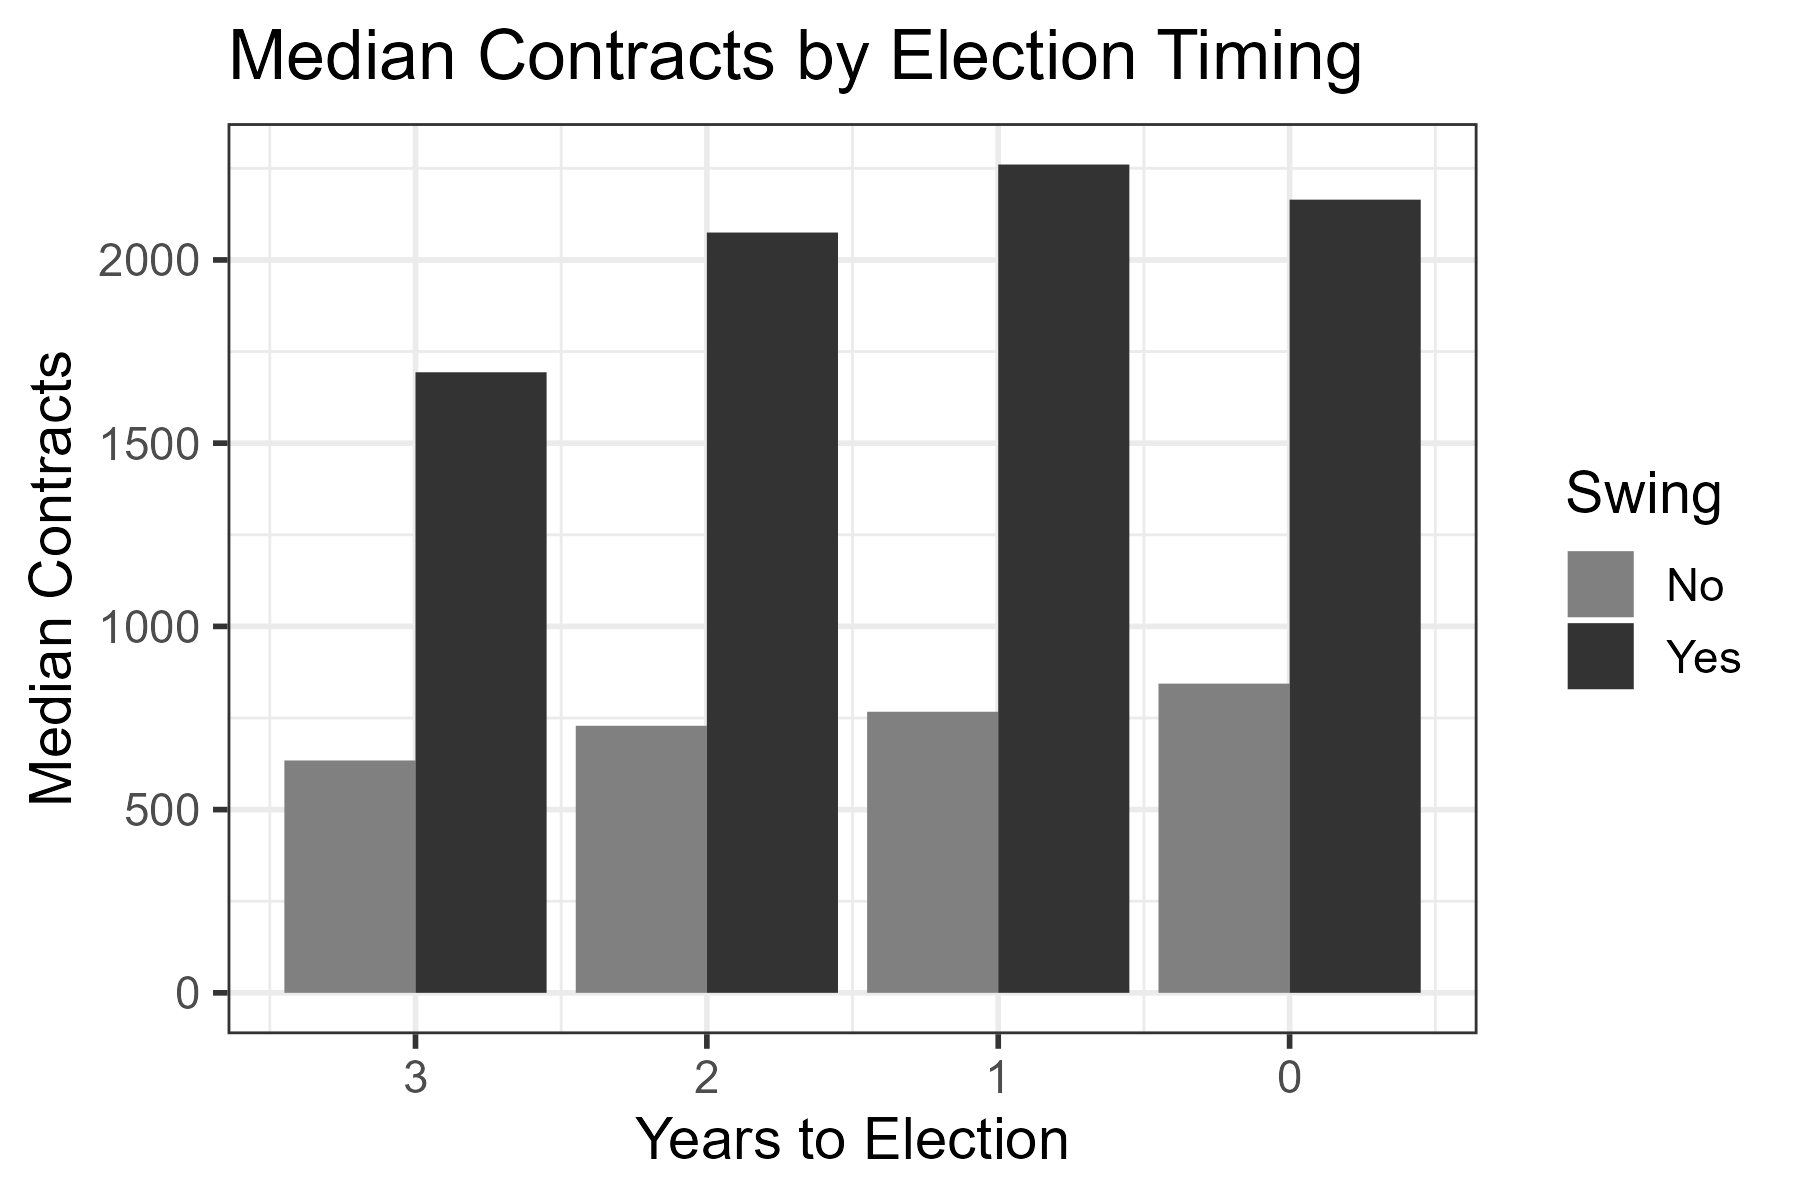
\includegraphics[width=0.95\textwidth]{cont-swing-raw.png}
	\caption{Median contracts in swing and non-swing states as presidential elections approach. I use the median because averages are sensitive to states with large or minimal arms contract awards. }
	\label{fig:cont-swing-raw}
\end{figure}


\subsection{Additional Estimates}


\autoref{fig:state-pars} presents estimates from the ordered beta regression with transformed contracts. 
There is wide variation in contracting levels and temporal dependence across states. 
States with higher contracting levels also have more consistent temporal autocorrelation in contracts, while states such as North Dakota receive occasional arms contracts and thus have little temporal dependence. 

\begin{figure}[htpb]
	\centering
		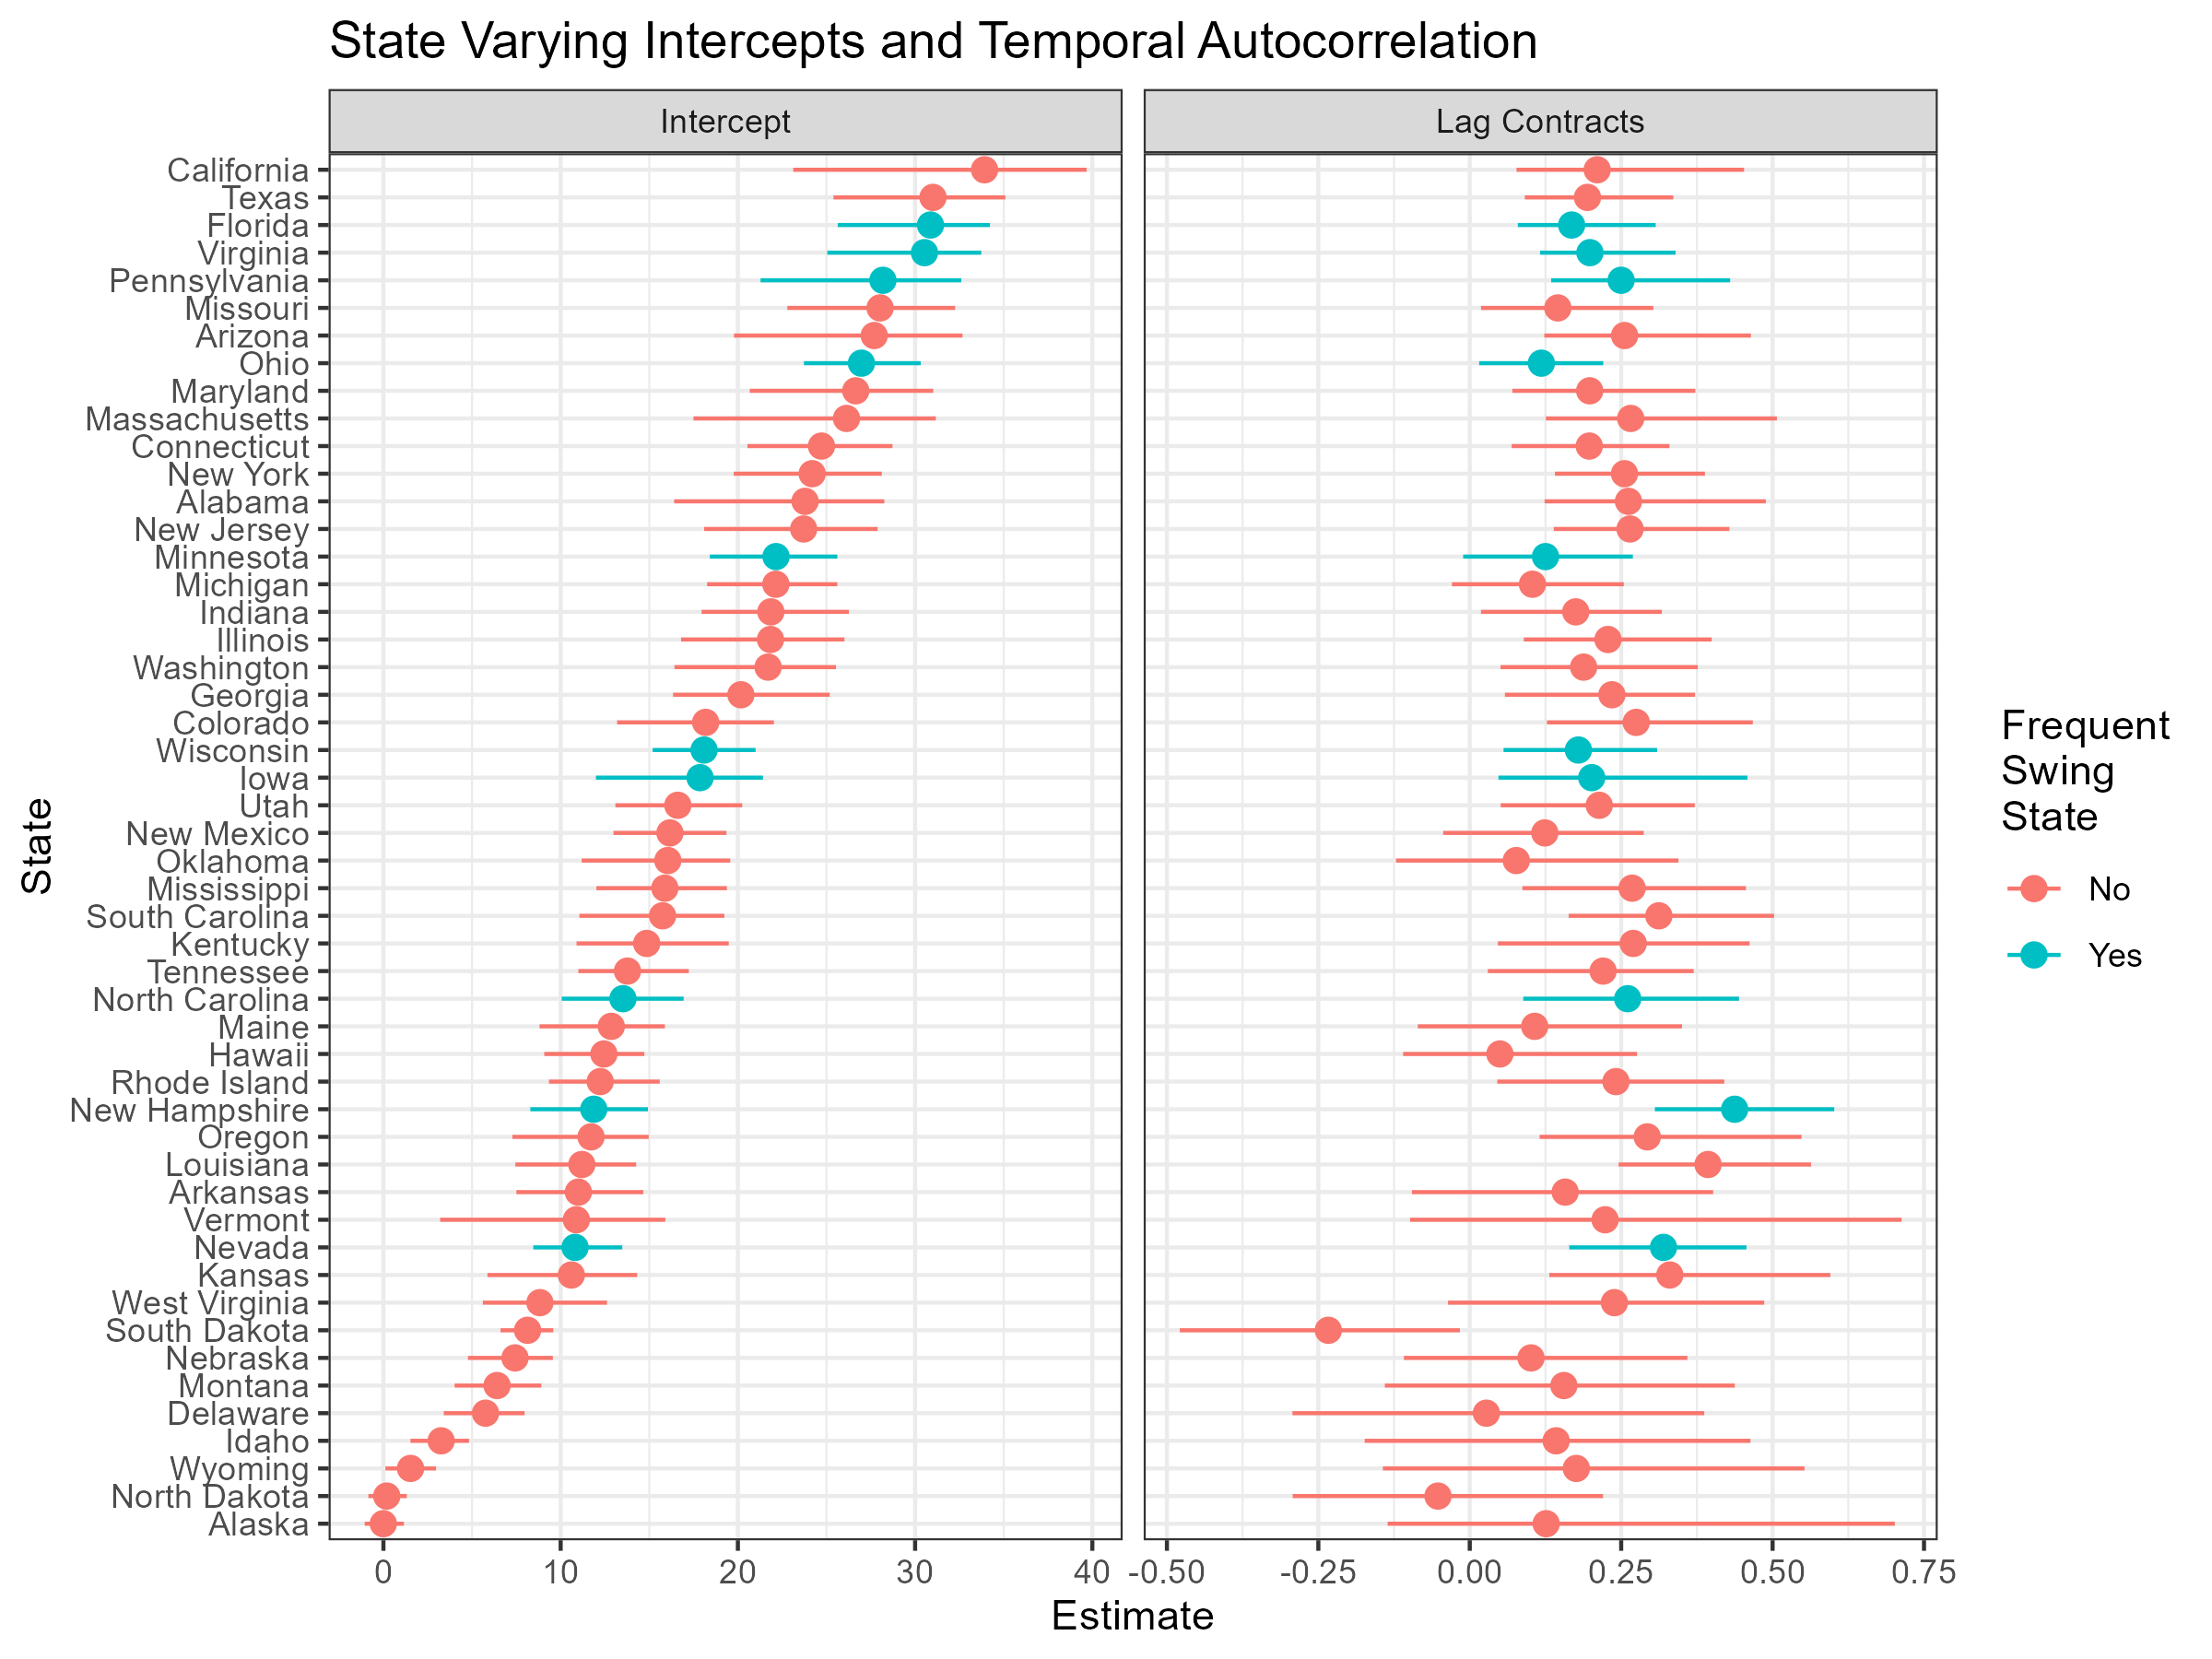
\includegraphics[width=0.95\textwidth]{state-pars.png}
	\caption{Estimated state intercept and temporal autocorrelation from ordered beta regression of transformed defense contracts in U.S. states, 2001-2020. Estimates ordered by the magnitude of the varying intercept. Error bars summarize the 90\% credible interval.}
	\label{fig:state-pars}
\end{figure}


\subsection{Alternative Estimators}

This section checks the results in the manuscript by adjusting the outcome measurement and estimation strategy in two ways.
First, I do not transform the contracts measure in any way, and fit a log-normal hurdle model, which assumes that the outcome has a zero process and observed values that are approximately normal after a log transformation. 
This approach does not model state-year observations with zero contracts well, but it fits non-zero contracts tolerably. 
As the top panel of \autoref{fig:me-deals-check} shows, the interaction between arms deals and swing state status is almost entirely positive.
At the same time, the association between deals and the level of contracts outside of swing states is almost entirely negative. 
This latter estimate is not part of the argument, and may be due to difficulties accounting for zeros in the log-normal hurdle. 
 

\begin{figure}[htpb]
	\centering
		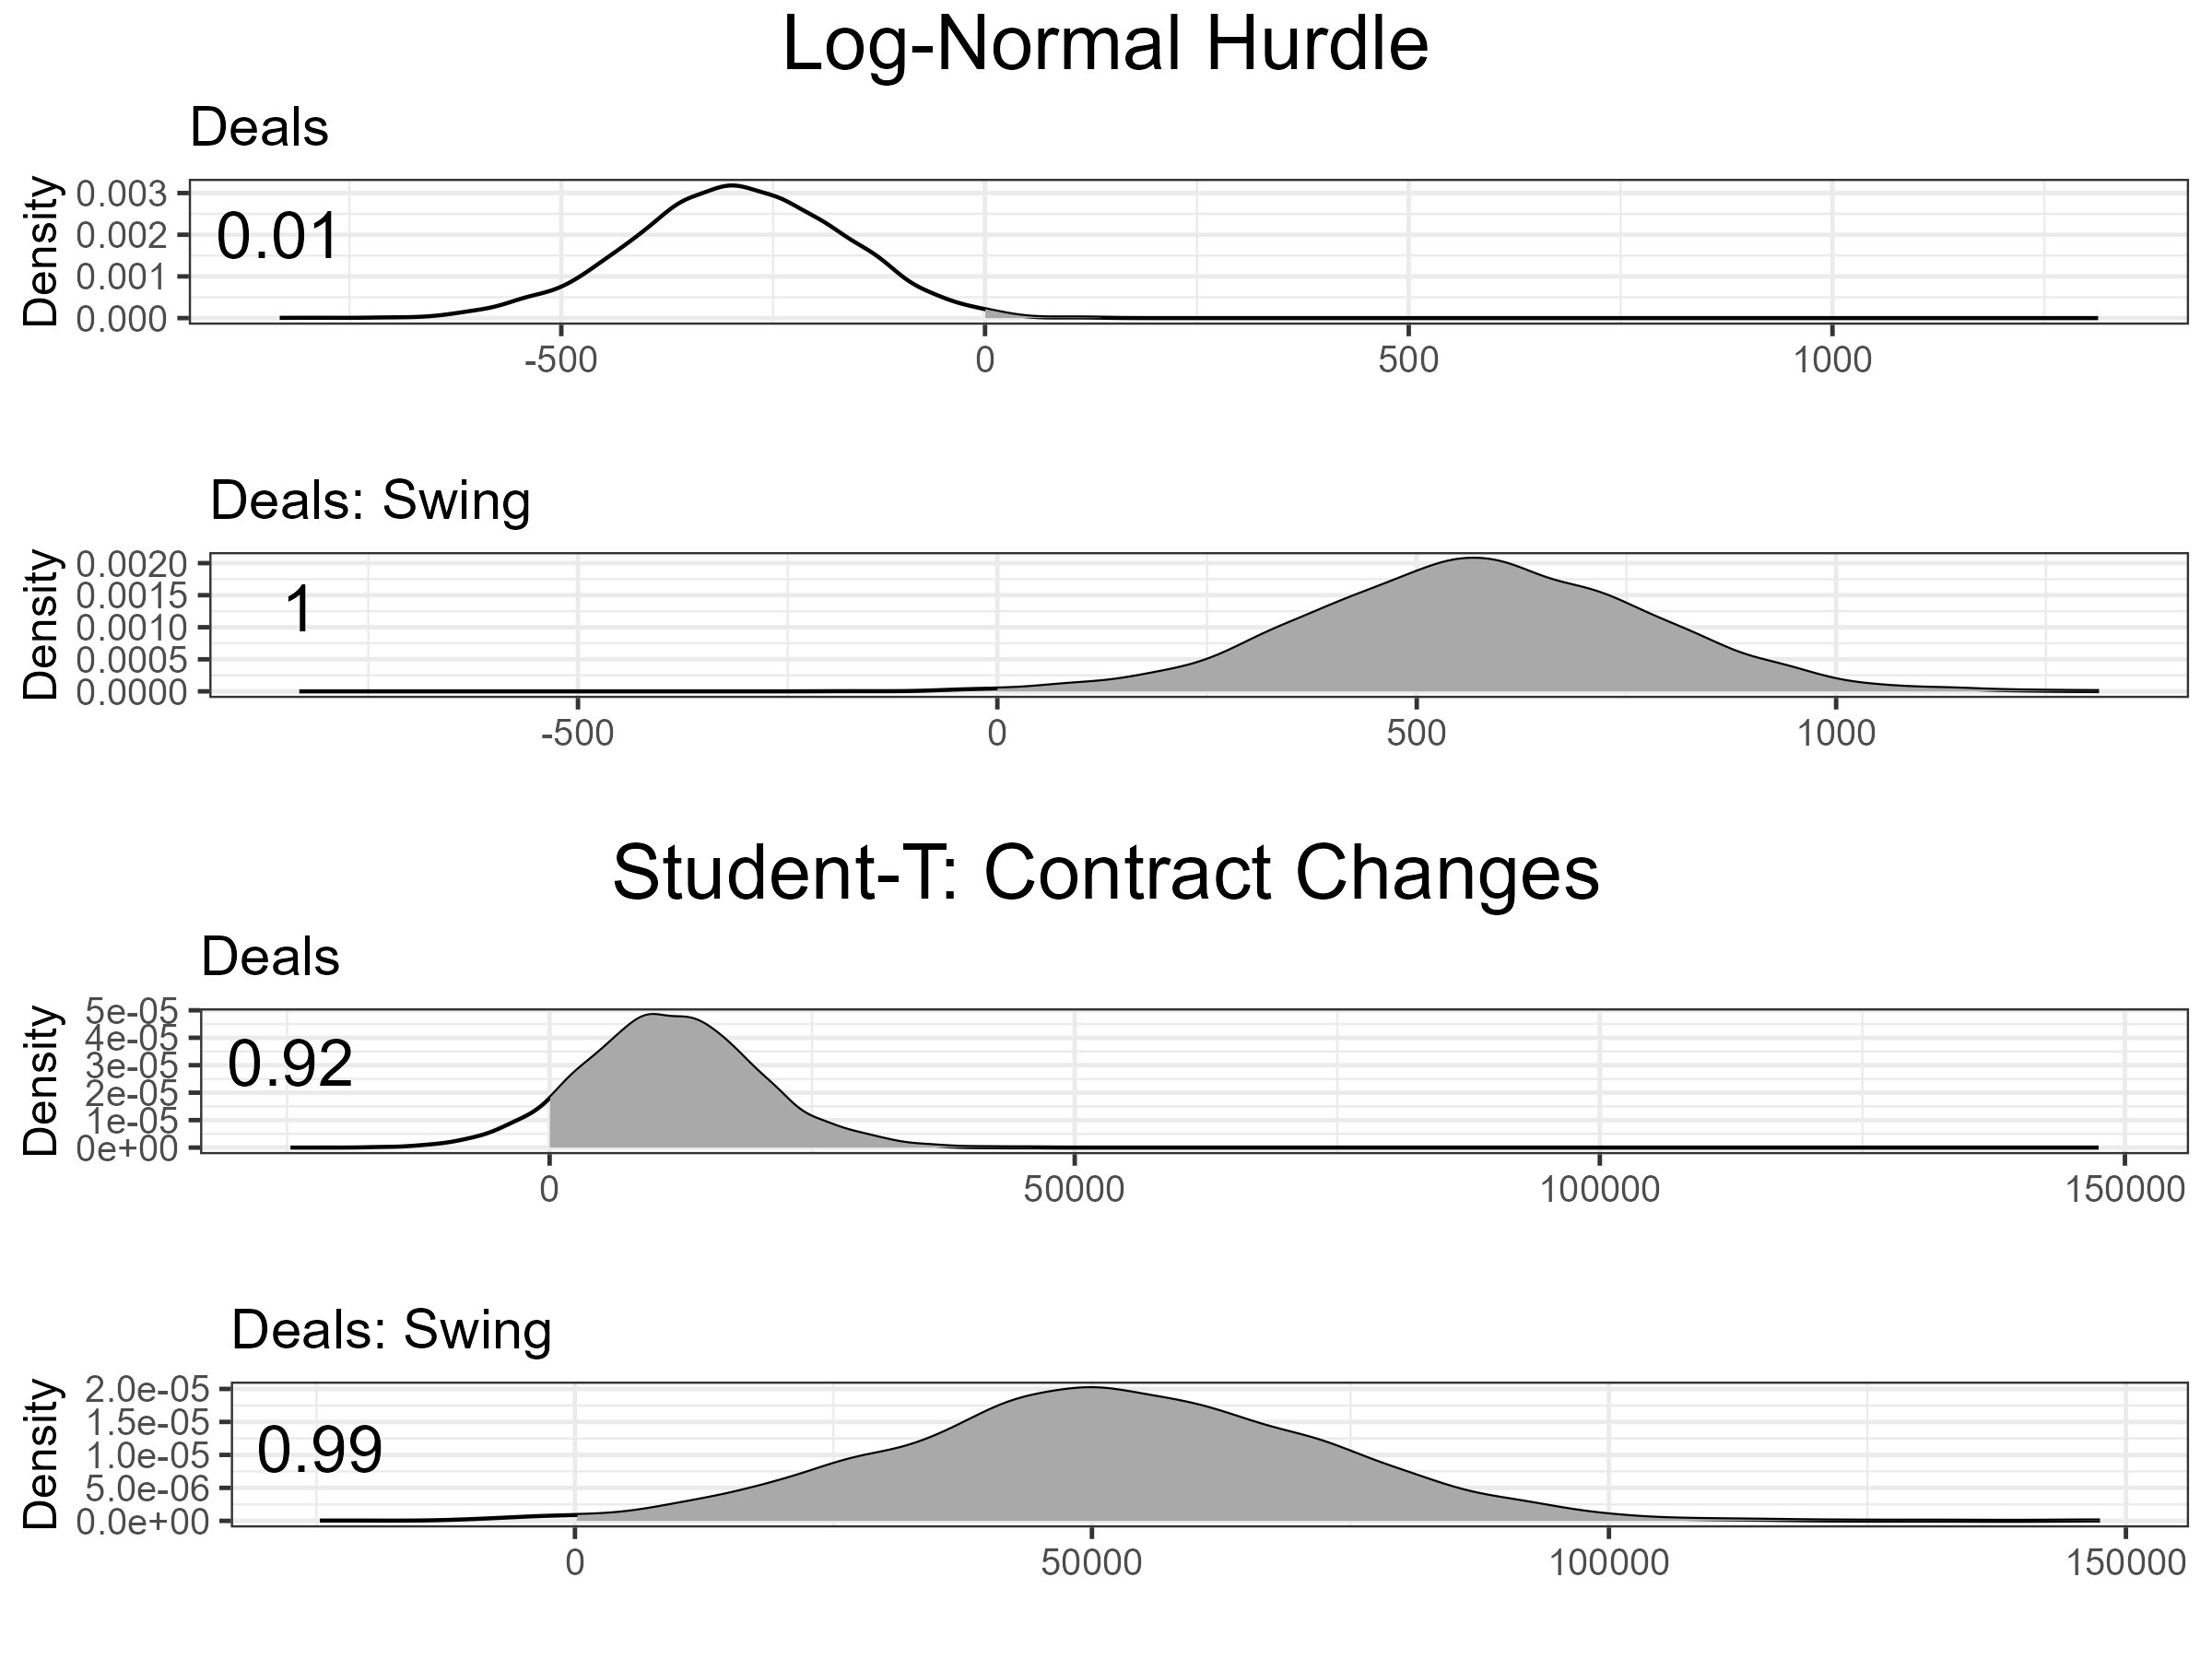
\includegraphics[width=0.95\textwidth]{me-deals-check.png}
	\caption{Shaded area and text give the positive posterior mass of each coefficient.}
	\label{fig:me-deals-check}
\end{figure}


A second approach uses the difference in contracts for each state in every year as the outcome. 
Because this measure is not normally distributed and has fat tails, I use a student-t outcome distribution.
The student-t model also omits the state-specific lagged dependent variable, because using changes eliminates some of those dynamics. 


Results from the student-t model of contract changes also suggest that arms deals increase contract awards to swing states. 
99\% of the posterior mass in the interaction coefficient between deals and states is positive.
While 92\% of the posterior mass in the deals term is positive, which suggests increased deals lead to increased changes in contracts for other states as well, there is a 95\% posterior probability that the relationship between arms deals and contracts in swing states is larger. 
As a result, arms deals increase changes in defense contracts more in swing states than in other states. 


%\newpage 

\section{Additional Mechanism}

Here, I document an additional check of the connection between deals and swing state contracts. 
The arms deals models show that deals with autocracies increase as presidential elections approach. 
If those deals go to swing state contracts, then the marginal impact of deals on contracts in swing states should increase as presidential elections approach. 


To check this, I alter the model of contracts in the manuscript by interacting the time to election indicator with swing state dummy and arms deals. 
I then present the marginal effect of deals on defense contracts in \autoref{fig:deals-me-prox}. 


\begin{figure}[htpb]
	\centering
		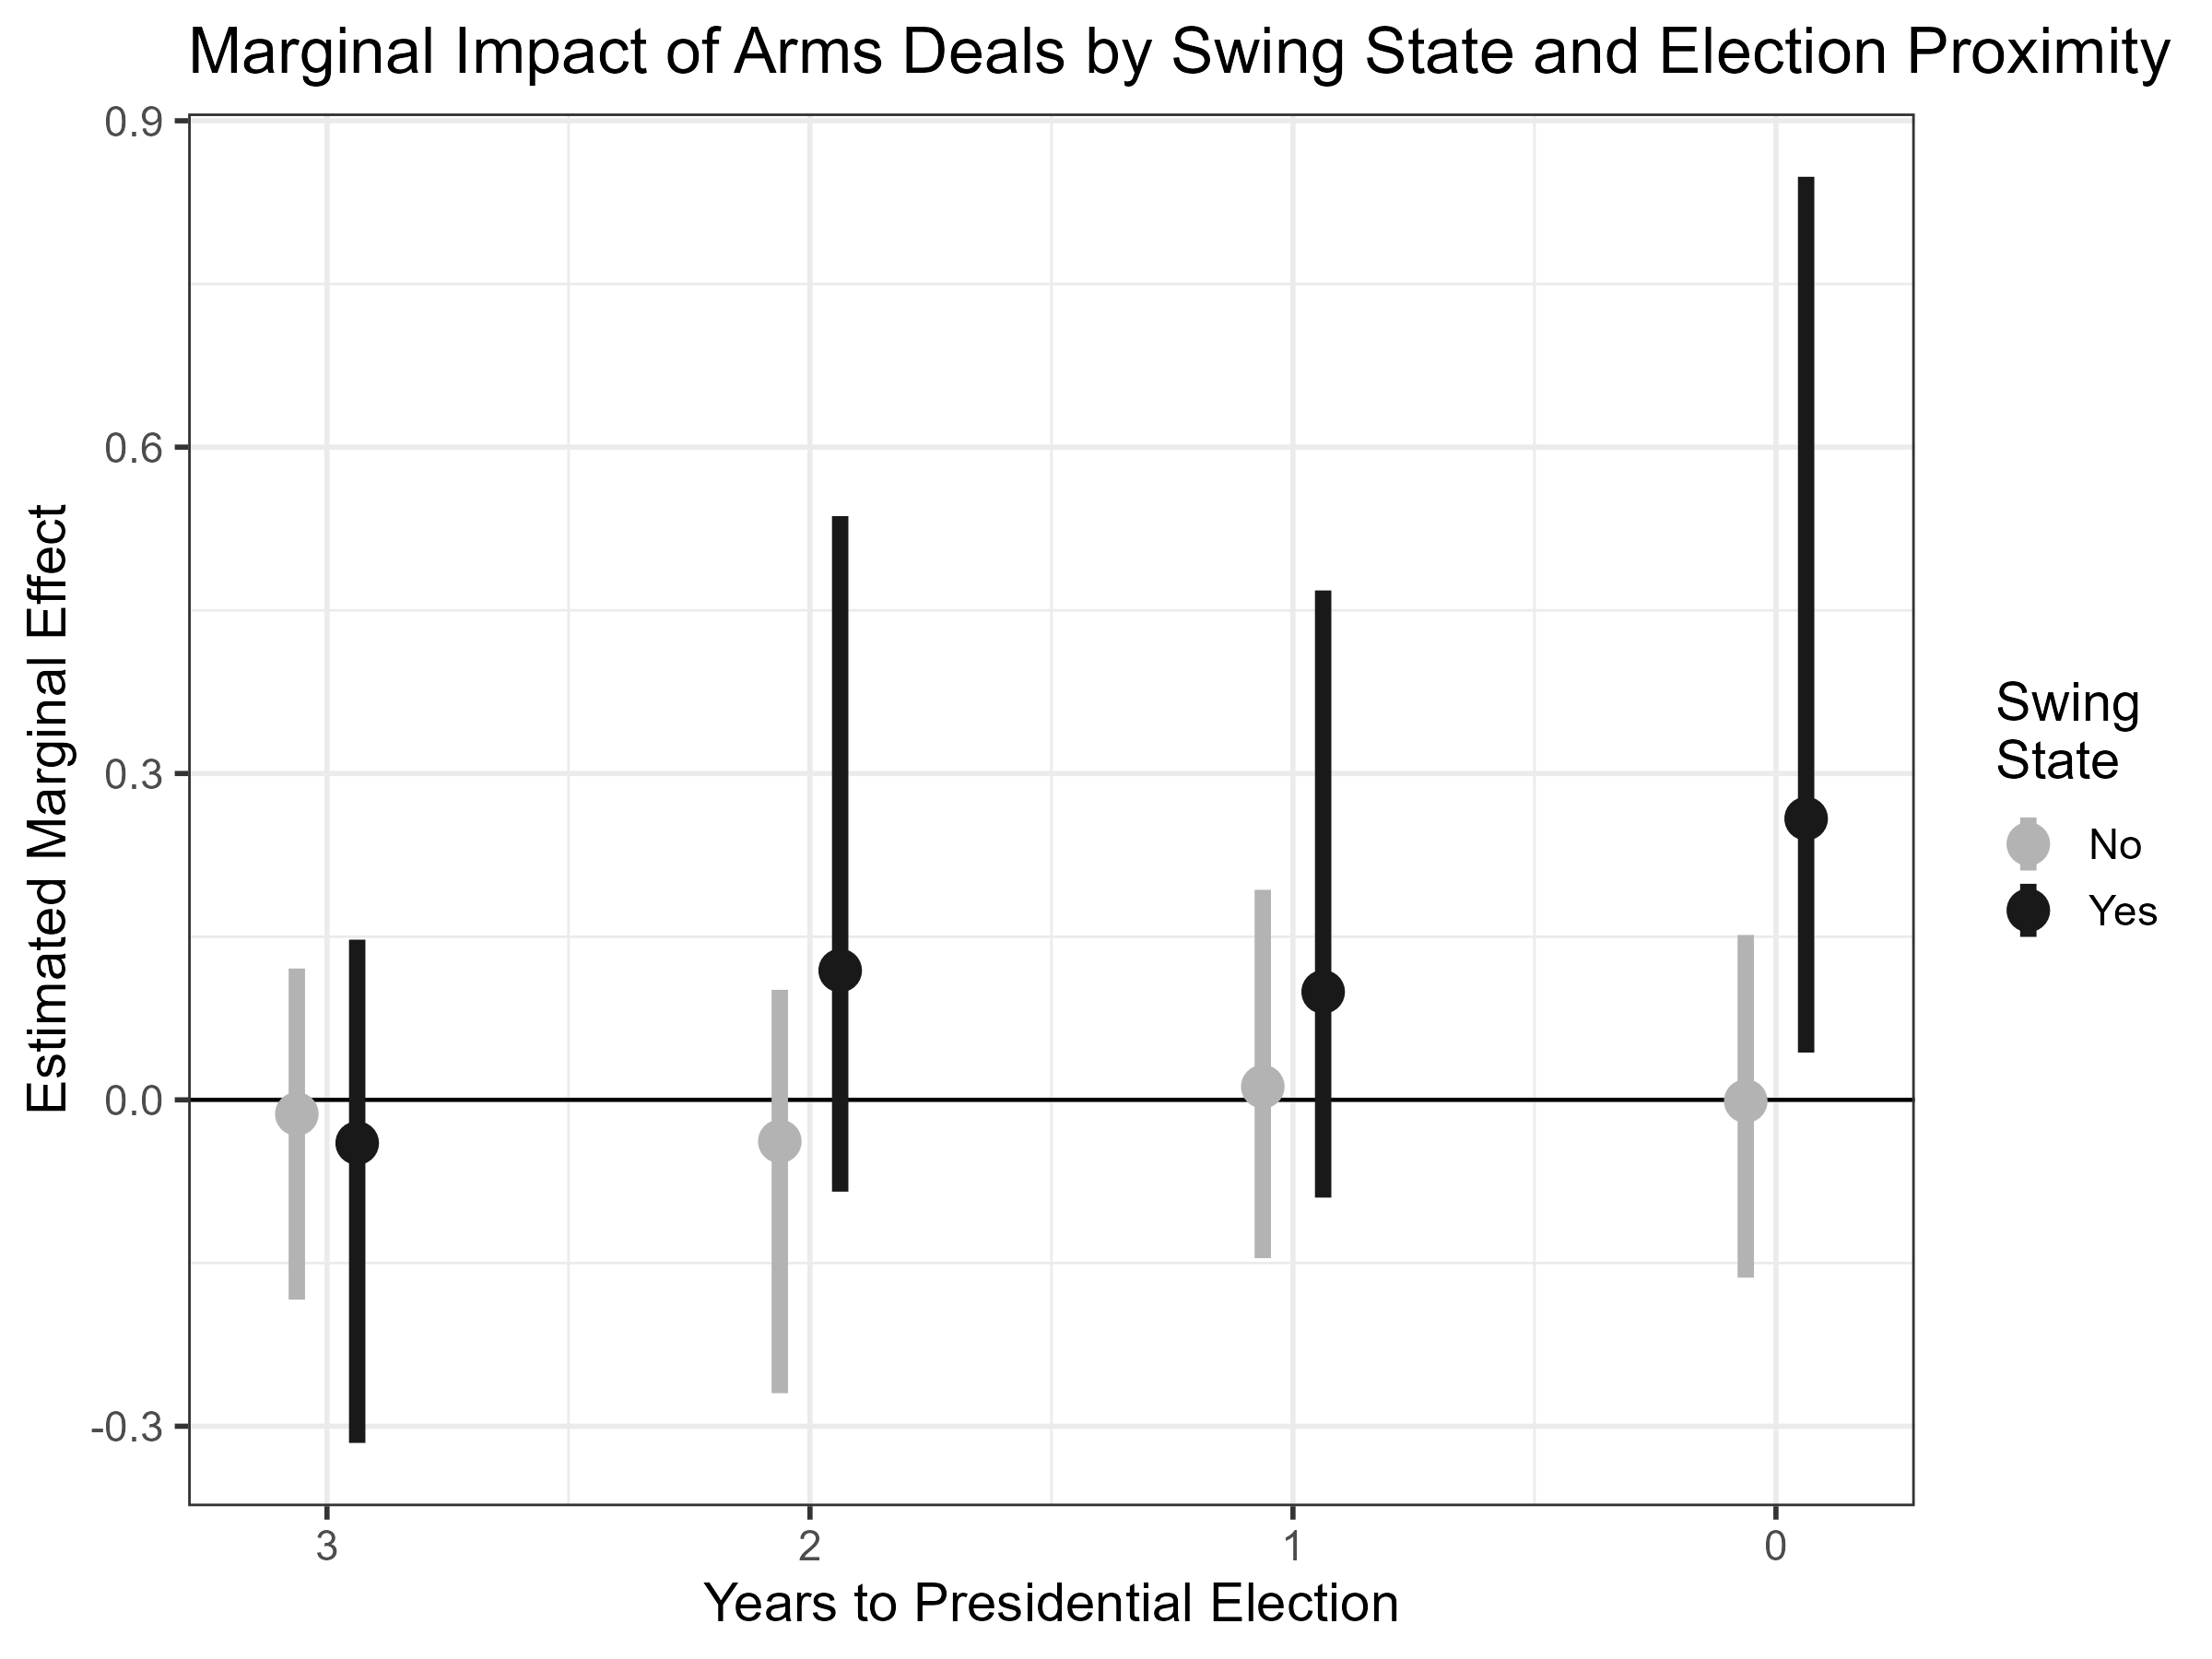
\includegraphics[width=0.95\textwidth]{deals-me-prox.png}
	\caption{Marginal effect of arms deals on defense contract awards based on swing state status and presidential election proximity. Estimates in millions of dollars.}
	\label{fig:deals-me-prox}
\end{figure}


The marginal impact of arms deals on contracts increases as presidential elections approach, but only in swing states. 
After an election, deals do not increase contracts in any state. 
But as a presidential election approaches, the marginal impact of deals on swing state contracts increases and is clearly positive in the year before and year of a presidential election. 
There is no clear impact of deals non-swing state contracts at any point in the electoral cycle. 
This implies that arms deals with autocracies near elections feed increased swing state contracts. 

%\newpage 

\section{Interaction Robustness}

The models in the manuscript use interactions that assume a linear functional form. 
Violations of linearity and other issues can generate misleading inferences \citep{Hainmuelleretal2019}. 
Here, I show that more flexible function forms give similar inferences about marginal effects. 
I do this by using binning estimators to examine the marginal impact of election proximity on arms deals and the marginal impact of swing state status on contracts.


First, I present the marginal effect of election proximity on arms deals in \autoref{fig:prox-deals-bin}.
When time to election is 0, the marginal impact of this relative to the year after a presidential election is largest states with a low polyarchy score. 
This is consistent with the argument, although comparisons at the other two levels are less so. 



\begin{figure}[htpb]
	\centering
		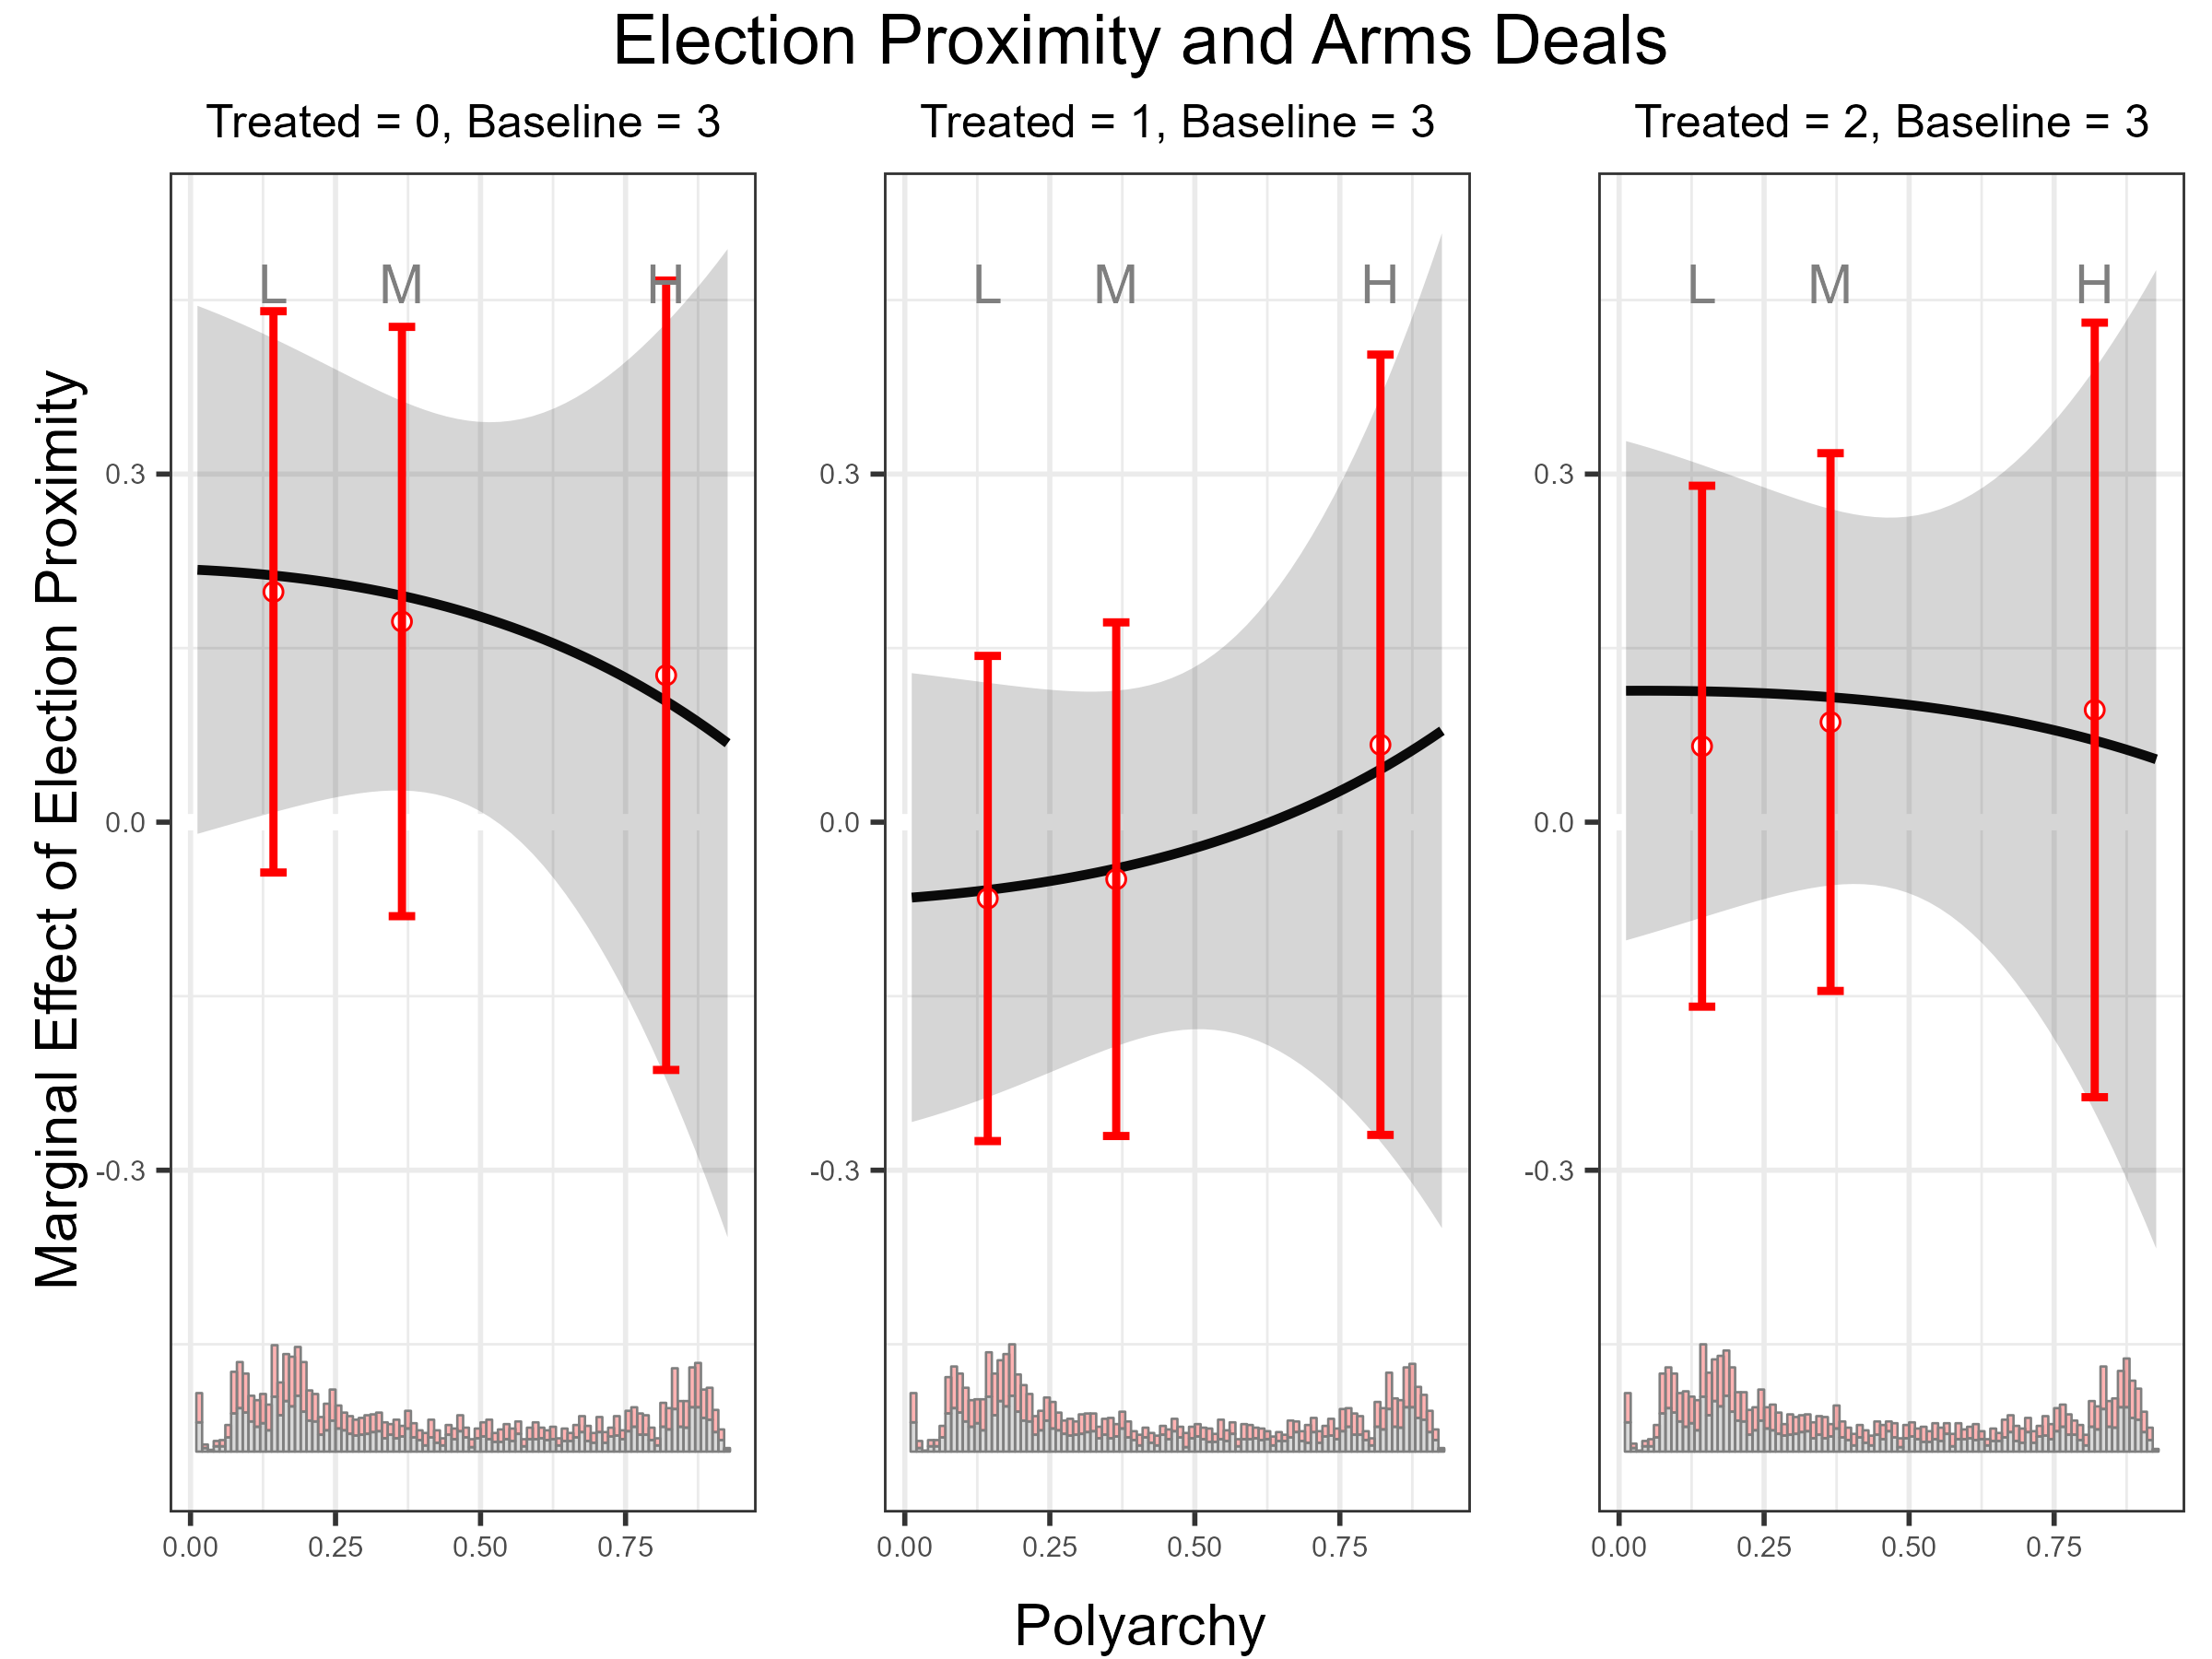
\includegraphics[width=0.95\textwidth]{prox-deals-bin.png}
	\caption{Marginal effect of election proximity on arms deals across the observed range of polyarchy. Each comparison uses three years to the presidential election as a baseline.}
	\label{fig:prox-deals-bin}
\end{figure}


Second, \autoref{fig:swing-cont-bin} shows the same pattern in the marginal impact of swing state status as the manuscript. 
As deals increase, so does the marginal effect of swing state status. 
Each bin deviates minimally from the linear relationship. 


\begin{figure}[htpb]
	\centering
		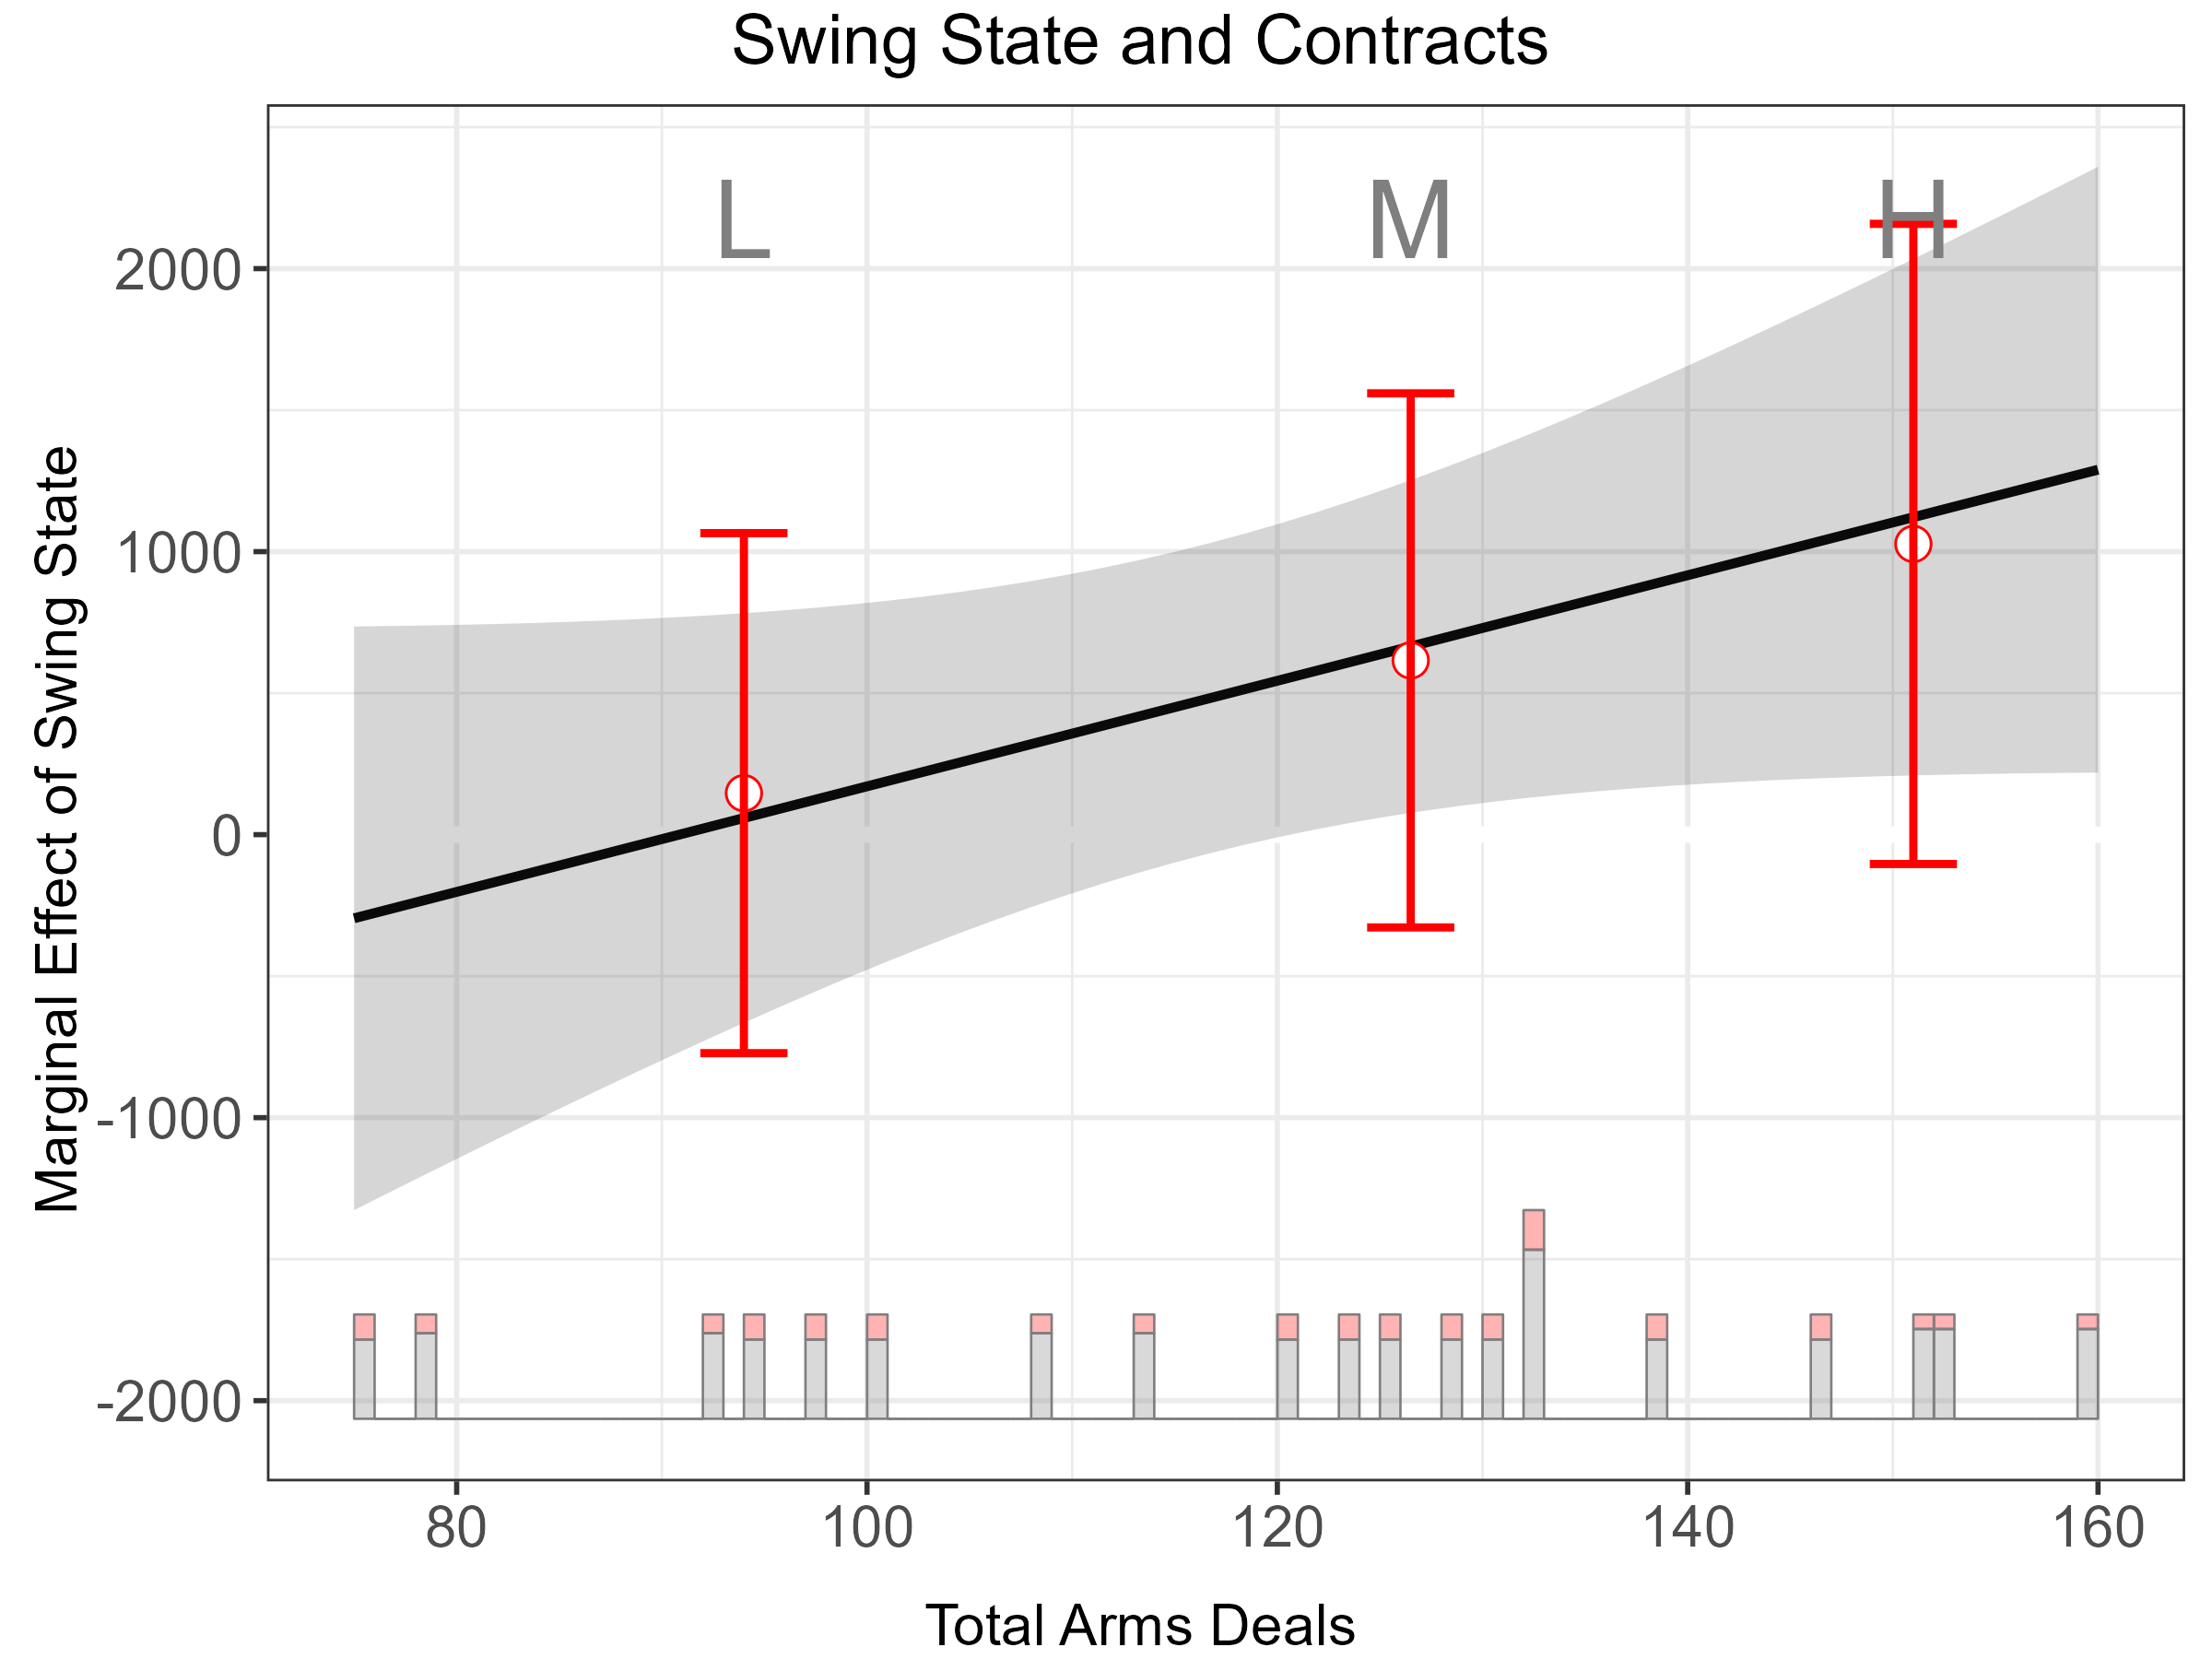
\includegraphics[width=0.95\textwidth]{swing-cont-bin.png}
	\caption{Marginal effect of swing state status on defense contract awards based on arms deals. Estimates in millions of dollars.}
	\label{fig:swing-cont-bin}
\end{figure}


\newpage

\section{Data Details}
\afterpage{\clearpage}
This section provides additional documentation, including tables of swing states, variables and sources, and coefficient estimates.  

\subsection{Swing State List}

\autoref{tab:swing-list} lists the set of swing states and the years they are swing states.
\begin{figure}[htpb]
	\centering
		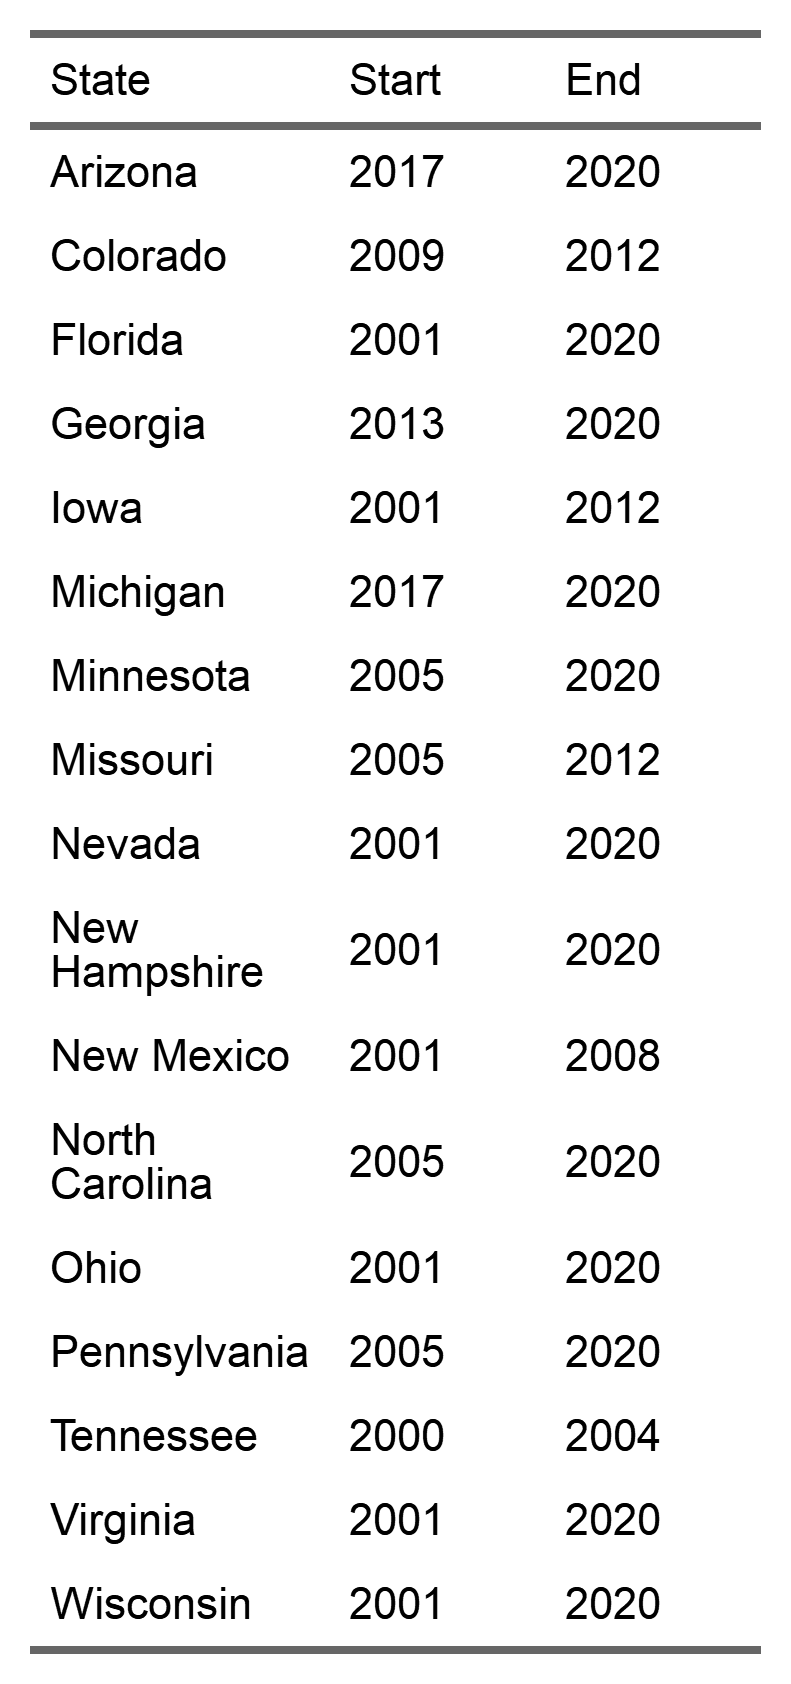
\includegraphics[width=5cm, height=10cm,keepaspectratio]{swing-list.png}
	\caption{List of swing states and years of swing status.}
	\label{tab:swing-list}
\end{figure}


\subsection{Variables and Sources}

\autoref{tab:deals-details} summarizes the variables and sources in the deals models. Some dyadic data from \citet{peacesciencer-package}. 
\autoref{tab:cont-details} does the same for variables in the contracting models. 

\begin{table}
\centering
\resizebox{\textwidth}{!}{%
\begin{tabular}[t]{lrrrrrrrr}
\toprule
  & Unique (\#) & Missing (\%) & Mean & SD & Min & Median & Max & Source\\
\midrule
Total Arms Deals & 27 & 0 & 0.9 & 2.3 & 0.0 & 0.0 & 48.0 & \citep{SIPRI2021} \\
Years to Election & 4 & 0 & 1.5 & 1.1 & 0.0 & 1.0 & 3.0 & Author\\
US Ally & 3 & 21 & 0.4 & 0.5 & 0.0 & 0.0 & 1.0 & \citep{Leedsetal2002} \& Author informal \\
Partner Polyarchy & 914 & 17 & 0.4 & 0.3 & 0.0 & 0.3 & 0.9 & \citep{Coppedgeetal2008} \\
Cold War & 2 & 0 & 0.6 & 0.5 & 0.0 & 1.0 & 1.0 & Author \\
Global War on Terror & 2 & 0 & 0.2 & 0.4 & 0.0 & 0.0 & 1.0 & Author \\
Republican President & 2 & 0 & 0.6 & 0.5 & 0.0 & 1.0 & 1.0 & Author\\
Log Petrol Revenue & 4742 & 37 & 11.4 & 10.6 & 0.0 & 16.5 & 27.1 & \citep{RossMahdavi2015} \\
Log Partner GDP & 10481 & 23 & 21.6 & 0.9 & 17.1 & 21.7 & 25.2 & \citep{Feenstraetal2015} \\
Ongoing MID & 3 & 30 & 0.0 & 0.2 & 0.0 & 0.0 & 1.0 & \citep{Palmeretal2021} \\
Log Partner Population & 11917 & 13 & 15.2 & 2.1 & 8.4 & 15.5 & 21.1  &\citep{Feenstraetal2015} \\
Log Pop. Weighted Distance) & 182 & 14 & 5.0 & 1.1 & 0.5 & 5.2 & 7.3 & \citep{FouquinHugot2016} \\
Common Language & 3 & 14 & 0.4 & 0.5 & 0.0 & 0.0 & 1.0 & \citep{FouquinHugot2016} \\
\bottomrule
\end{tabular}
}
\caption{Variables and data sources in arms deals models}
\label{tab:deals-details}
\end{table}


\begin{table}
\centering
\resizebox{\textwidth}{!}{%
\begin{tabular}[t]{lrrrrrrrr}
\toprule
  & Unique (\#) & Missing (\%) & Mean & SD & Min & Median & Max & Source\\
\midrule
Contracts & 948 & 5 & 2761.0 & 4703.9 & 0.0 & 907.3 & 56290.7 & \href{https://www.usaspending.gov/download_center/award_data_archive}{USASpending.gov} \\
Lag Contracts & 900 & 5 & 2552.6 & 4314.5 & 0.0 & 782.0 & 34204.8 & Author \\
Arms Deals & 20 & 0 & 120.1 & 23.4 & 75.0 & 125.0 & 160.0 & \citep{SIPRI2021} \\
Swing State & 2 & 0 & 0.2 & 0.4 & 0.0 & 0.0 & 1.0 & \citep{KrinerReeves2015} \\
Core State & 2 & 0 & 0.3 & 0.4 & 0.0 & 0.0 & 1.0  & \citep{KrinerReeves2015} \\
Global War
on Terror & 2 & 0 & 0.5 & 0.5 & 0.0 & 1.0 & 1.0 & Author \\
Time to Election & 4 & 0 & 1.4 & 1.1 & 0.0 & 1.0 & 3.0 & Author \\
Republican President & 2 & 0 & 0.6 & 0.5 & 0.0 & 1.0 & 1.0 & Author \\
Population (Rescaled) & 1000 & 0 & 0.0 & 0.5 & -1.2 & 0.1 & 1.1 & \citep{Grossmannetal2021} \\
Log GDP (Rescaled) & 1050 & 0 & -0.0 & 0.5 & -1.4 & 0.0 & 1.1 & FRED (St. Louis Federal Reserve) \\
\bottomrule
\end{tabular}
}
\caption{Variables and data sources in defense contracting models}
\label{tab:cont-details}
\end{table}


\subsection{Coefficient Estimates}

The section presents tables with coefficient estimates. 
\autoref{tab:pois-regs} summarizes the hurdle Poisson coefficient estimates for the aggregate deals model, while \autoref{tab:pois-regs-sector} summarizes the models of arms deals by type.\footnote{All tables built with modelsummary \citep{ArelBundock2022}}. 
\autoref{tab:cont-regs} summarizes the three deals models and \autoref{tab:cont-regs-sector} gives ordered-beta coefficient estimates for the sectoral models of defense contracts. 


\begin{table}[H]

\caption{\label{tab:pois-regs}: Coefficient estimates from Poisson models of US arms deals.}
\centering
\resizebox{\linewidth}{!}{
\fontsize{8}{10}\selectfont
\begin{tabular}[t]{lcccc}
\toprule
  & Generic Cycle & Regime Cycle (No Controls) & Regime Cycle & Regime and Ally Cycle\\
\midrule
Hurdle: Intercept & 6 &  & 5 & 5\\
 & (4, 7) &  & (3, 6) & (3, 6)\\
Intercept & -1.0 & -0.13 & -0.8 & -0.66\\
 & (-1.5, -0.4) & (-0.19, -0.06) & (-1.4, -0.2) & (-1.28, -0.04)\\
Years to Election & -0.03 & -0.07 & -0.09 & -0.17\\
 & (-0.05, -0.01) & (-0.11, -0.03) & (-0.13, -0.06) & (-0.24, -0.09)\\
US Ally & 0.8 &  & 0.8 & 0.6\\
 & (0.7, 0.8) &  & (0.8, 0.9) & (0.4, 0.7)\\
Polyarchy & -0.07 & 0.9 & -0.2 & -0.6\\
 & (-0.15, 0.01) & (0.8, 1.0) & (-0.3, -0.1) & (-0.9, -0.3)\\
Cold War & 0.2 &  & 0.2 & 0.2\\
 & (0.1, 0.3) &  & (0.1, 0.3) & (0.1, 0.3)\\
Global War on Terror & -0.15 &  & -0.15 & -0.15\\
 & (-0.23, -0.07) &  & (-0.23, -0.07) & (-0.23, -0.07)\\
EU Member & 0.2 &  &  & \\
 & (0.1, 0.3) &  &  & \\
Republican President & -0.009 &  & -0.02 & -0.02\\
 & (-0.053, 0.037) &  & (-0.06, 0.03) & (-0.06, 0.03)\\
Log GDP & -0.04 &  & -0.030 & -3e-02\\
 & (-0.06, -0.01) &  & (-0.056, -0.003) & (-5e-02, -7e-04)\\
Ongoing MID & -0.23 &  & -0.3 & -0.3\\
 & (-0.42, -0.05) &  & (-0.5, -0.1) & (-0.5, -0.1)\\
Log Population & 0.2 &  & 0.2 & 0.2\\
 & (0.2, 0.2) &  & (0.1, 0.2) & (0.1, 0.2)\\
Log Distance & -0.07 &  & -0.12 & -0.11\\
 & (-0.10, -0.04) &  & (-0.15, -0.09) & (-0.14, -0.08)\\
Common Language & 0.03 &  & 4e-02 & 0.048\\
 & (-0.01, 0.08) &  & (5e-05, 9e-02) & (0.006, 0.091)\\
Hurdle: US Ally & -2 &  & -2 & -2\\
 & (-2, -2) &  & (-2, -2) & (-2, -2)\\
Hurdle: Polyarchy & 0.5 &  & 0.4 & 0.4\\
 & (0.3, 0.7) &  & (0.2, 0.6) & (0.2, 0.6)\\
Hurdle: Ongoing MID & 0.7 &  & 0.6 & 0.7\\
 & (0.3, 1.1) &  & (0.2, 1.1) & (0.3, 1.1)\\
Hurdle: Log GDP & -0.2 &  & -0.16 & -0.16\\
 & (-0.3, -0.1) &  & (-0.23, -0.08) & (-0.23, -0.08)\\
Years to Election:Polyarchy &  & 0.068 & 0.11 & 0.17\\
 &  & (0.009, 0.129) & (0.05, 0.17) & (-0.01, 0.35)\\
Log Petrol Revenue &  &  & 0.010 & 0.009\\
 &  &  & (0.007, 0.013) & (0.006, 0.012)\\
Years to Election:US Ally &  &  &  & 0.10\\
 &  &  &  & (0.01, 0.19)\\
US Ally:Polyarchy &  &  &  & 0.5\\
 &  &  &  & (0.1, 0.8)\\
Years to Election:US Ally:Polyarchy &  &  &  & -0.09\\
 &  &  &  & (-0.28, 0.10)\\
\bottomrule
\multicolumn{5}{l}{\rule{0pt}{1em}\textit{Note: }}\\
\multicolumn{5}{l}{\rule{0pt}{1em}90\% Credible Intervals in parentheses.}\\
\end{tabular}}
\end{table}

\afterpage{\clearpage}
\begin{table}

\caption{\label{tab:pois-regs-sector}: Coefficient estimates from hurdle Poisson models of US arms deals by sector.}
\centering
\resizebox{\linewidth}{!}{
\fontsize{8}{10}\selectfont
\begin{tabular}[t]{lcccccc}
\toprule
  & Aircraft & Arms & Electronics & Missile and Space & Ships & Vehicles\\
\midrule
Hurdle: Intercept & 6.0 & 5.9 & 7.9 & 6.5 & 8.7 & 6.0\\
 & (4.3, 7.7) & (2.9, 9.0) & (4.7, 11.2) & (3.9, 9.2) & (5.6, 11.9) & (3.4, 8.6)\\
Intercept & -0.24 & -0.00061 & -0.071 & -0.25 & 0.17 & -0.27\\
 & (-0.97, 0.49) & (-0.94533, 0.95467) & (-1.051, 0.866) & (-1.20, 0.65) & (-0.75, 1.08) & (-1.22, 0.65)\\
Years to Election & -0.039 & -0.153 & -0.096 & -0.188 & -0.47 & -0.099\\
 & (-0.175, 0.087) & (-0.414, 0.096) & (-0.374, 0.168) & (-0.390, 0.013) & (-0.83, -0.15) & (-0.275, 0.071)\\
US Ally & 1.01 & 0.20 & 0.069 & 0.025 & 0.543 & -0.032\\
 & (0.79, 1.25) & (-0.32, 0.71) & (-0.461, 0.578) & (-0.380, 0.422) & (0.062, 1.061) & (-0.390, 0.311)\\
Polyarchy & -0.0058 & 0.34 & -0.16 & -0.25 & -0.42 & 0.40\\
 & (-0.4681, 0.4434) & (-0.30, 0.97) & (-0.80, 0.51) & (-0.84, 0.32) & (-1.16, 0.32) & (-0.19, 0.93)\\
Cold War & 0.27 & 0.316 & 0.65 & 0.25 & 0.54 & 0.1768\\
 & (0.18, 0.36) & (0.048, 0.582) & (0.40, 0.88) & (0.11, 0.40) & (0.27, 0.84) & (-0.0089, 0.3705)\\
EU Member & 0.28 & 0.80 & 0.63 & 0.31 & 0.474 & 0.63\\
 & (0.14, 0.42) & (0.48, 1.11) & (0.31, 0.93) & (0.13, 0.48) & (0.025, 0.921) & (0.38, 0.88)\\
Republican President & -0.0704 & -0.063 & -0.06 & -0.047 & 0.238 & -0.0049\\
 & (-0.1359, -0.0037) & (-0.279, 0.159) & (-0.28, 0.15) & (-0.178, 0.079) & (0.059, 0.421) & (-0.1511, 0.1464)\\
Log GDP & -0.066 & -0.019 & -0.095 & -0.031 & -0.055 & -0.0022\\
 & (-0.101, -0.033) & (-0.099, 0.059) & (-0.177, -0.016) & (-0.085, 0.024) & (-0.134, 0.019) & (-0.0617, 0.0594)\\
Ongoing MID & -0.287 & -0.16 & -0.31 & 0.04 & -0.12 & -0.044\\
 & (-0.575, -0.022) & (-0.90, 0.48) & (-1.12, 0.41) & (-0.51, 0.51) & (-0.94, 0.61) & (-0.580, 0.409)\\
Log Population & 0.067 & -0.023 & 0.059 & 0.12 & -0.020 & 0.0077\\
 & (0.034, 0.100) & (-0.132, 0.089) & (-0.042, 0.159) & (0.05, 0.18) & (-0.119, 0.081) & (-0.0699, 0.0818)\\
Log Distance & 0.075 & 0.04 & 0.151 & -0.154 & 0.159 & 0.048\\
 & (0.028, 0.121) & (-0.10, 0.18) & (0.014, 0.292) & (-0.236, -0.072) & (0.029, 0.292) & (-0.056, 0.152)\\
Common Language & 0.21 & 0.2083 & 0.18 & -0.015 & 0.088 & 0.13\\
 & (0.14, 0.28) & (-0.0012, 0.4185) & (-0.04, 0.39) & (-0.147, 0.117) & (-0.091, 0.262) & (-0.01, 0.27)\\
Years to Election:US Ally & 0.006 & 0.299 & 0.016 & 0.167 & 0.360 & 0.068\\
 & (-0.132, 0.145) & (0.011, 0.602) & (-0.296, 0.336) & (-0.069, 0.420) & (0.013, 0.725) & (-0.136, 0.280)\\
Years to Election:Polyarchy & 0.014 & 0.18 & -0.21 & 0.048 & -0.18 & -0.045\\
 & (-0.262, 0.287) & (-0.27, 0.60) & (-0.72, 0.28) & (-0.342, 0.445) & (-0.85, 0.44) & (-0.433, 0.342)\\
US Ally:Polyarchy & -0.14 & 0.059 & 0.40 & 0.615 & 0.031 & -0.092\\
 & (-0.59, 0.35) & (-0.611, 0.716) & (-0.26, 1.09) & (0.019, 1.220) & (-0.685, 0.734) & (-0.671, 0.555)\\
Years to Election:US Ally:Polyarchy & -0.0085 & -0.442 & 0.25 & 0.0088 & 0.32 & 0.17\\
 & (-0.2921, 0.2746) & (-0.895, 0.044) & (-0.25, 0.78) & (-0.4138, 0.4307) & (-0.31, 0.99) & (-0.24, 0.57)\\
Hurdle: US Ally & -2.0 & -2.0 & -2.2 & -2.4 & -2.9 & -1.9\\
 & (-2.1, -1.9) & (-2.2, -1.8) & (-2.4, -1.9) & (-2.5, -2.2) & (-3.1, -2.6) & (-2.1, -1.7)\\
Hurdle: Ongoing MID & 0.510 & 0.32 & 0.77 & 0.47 & 1.17 & 0.20\\
 & (0.064, 0.963) & (-0.40, 1.26) & (-0.15, 2.06) & (-0.21, 1.24) & (0.12, 2.63) & (-0.40, 0.85)\\
Hurdle: Log GDP & -0.18 & -0.117 & -0.197 & -0.153 & -0.215 & -0.139\\
 & (-0.26, -0.11) & (-0.259, 0.023) & (-0.347, -0.047) & (-0.275, -0.031) & (-0.362, -0.072) & (-0.263, -0.019)\\
\bottomrule
\multicolumn{7}{l}{\rule{0pt}{1em}\textit{Note: }}\\
\multicolumn{7}{l}{\rule{0pt}{1em}90\% Credible Intervals in parentheses.}\\
\end{tabular}}
\end{table}


\begingroup\fontsize{8}{10}\selectfont

\begin{longtable}[t]{lccc}
\caption{\label{tab:cont-regs}: Coefficient estimates from models of defense contract awards.}\\
\toprule
  & Rescaled Ordered Beta & Log-Normal Hurdle & Student-T: Contract Changes\\
\midrule
Intercept & -5.1 & 6.3 & 0.31\\
 & (-5.6, -4.6) & (5.7, 6.8) & (-3.56, 4.15)\\
Arms Deals & -0.00026 & -0.00209 & 0.081\\
 & (-0.00155, 0.00103) & (-0.00389, -0.00041) & (-0.033, 0.205)\\
Swing State & -0.290 & -0.56 & 0.079\\
 & (-0.535, -0.034) & (-0.92, -0.21) & (-3.901, 4.106)\\
Core State & 0.0424 & 0.079 & 0.016\\
 & (-0.0041, 0.0906) & (0.012, 0.146) & (-3.667, 3.806)\\
Global War on Terror & 0.013 & 0.26 & 0.76\\
 & (-0.058, 0.082) & (0.18, 0.35) & (-3.14, 4.62)\\
Time to Election & 0.00092 & -0.045 & 0.05\\
 & (-0.01649, 0.01748) & (-0.068, -0.022) & (-3.52, 3.57)\\
Republican President & 0.029 & -0.0082 & 1.2\\
 & (-0.024, 0.079) & (-0.0762, 0.0582) & (-2.7, 5.1)\\
Population (Rescaled) & 0.098 & -0.011 & -0.35\\
 & (-0.011, 0.207) & (-0.127, 0.106) & (-4.18, 3.52)\\
Log GDP & -0.082 & 0.37 & -0.24\\
 & (-0.181, 0.019) & (0.25, 0.49) & (-4.15, 3.59)\\
Arms Deals:Swing State & 1.9e-03 & 0.0041 & 0.367\\
 & (6.1e-06, 3.9e-03) & (0.0013, 0.0068) & (0.083, 0.647)\\
$\phi$ & 629 &  & \\
 & (565, 698) &  & \\
Hurdle: Intercept &  & -2.9 & \\
 &  & (-3.2, -2.6) & \\
Hurdle: Log GDP &  & -0.659 & \\
 &  & (-1.228, -0.065) & \\
$\sigma$ &  & 0.38 & 135\\
 &  & (0.37, 0.40) & (121, 151)\\
\bottomrule
\multicolumn{4}{l}{\rule{0pt}{1em}\textit{Note: }}\\
\multicolumn{4}{l}{\rule{0pt}{1em}90\% Credible Intervals in parentheses.}\\
\end{longtable}
\endgroup{}


\begin{table}

\caption{\label{tab:cont-regs-sector}: Coefficient estimates from models of defense contract awards by sector.}
\centering
\resizebox{\linewidth}{!}{
\fontsize{8}{10}\selectfont
\begin{tabular}[t]{lcccccc}
\toprule
  & Aircraft & Arms & Electronics & Missile and Space & Ships & Vehicles\\
\midrule
Intercept & -5 & -5 & -5 & -6 & -5 & -5\\
 & (-6, -5) & (-5, -4) & (-6, -5) & (-6, -5) & (-6, -5) & (-5, -5)\\
Aircraft Deals & -3e-04 &  &  &  &  & \\
 & (-3e-03, 2e-03) &  &  &  &  & \\
Swing State & -0.37 & -0.23 & -0.08 & 0.23 & 0.1 & 0.08\\
 & (-0.66, -0.09) & (-0.50, 0.03) & (-0.22, 0.05) & (-0.02, 0.49) & (-0.1, 0.4) & (-0.17, 0.35)\\
Core State & -0.01 & 0.08 & 0.02 & -0.02 & 0.08 & 0.3\\
 & (-0.07, 0.04) & (-0.01, 0.18) & (-0.03, 0.08) & (-0.10, 0.05) & (-0.01, 0.16) & (0.1, 0.4)\\
Global War on Terror & 0.06 & 0.10 & 0.002 & 0.07 & -0.04 & -0.004\\
 & (-0.02, 0.15) & (-0.02, 0.22) & (-0.072, 0.075) & (-0.04, 0.17) & (-0.15, 0.07) & (-0.132, 0.125)\\
Republican President & -0.02 & 0.01 & -0.02 & -0.06 & 0.04 & -0.113\\
 & (-0.10, 0.05) & (-0.07, 0.10) & (-0.06, 0.03) & (-0.15, 0.04) & (-0.04, 0.12) & (-0.229, 0.004)\\
Log GDP & 0.10 & 0.12 & 0.15 & 0.02 & -0.2 & 0.01\\
 & (-0.03, 0.22) & (-0.07, 0.31) & (0.04, 0.28) & (-0.18, 0.21) & (-0.4, -0.1) & (-0.19, 0.21)\\
Population (Rescaled) & -0.002 & -0.03 & -0.12 & -0.008 & 0.178 & -0.09\\
 & (-0.149, 0.144) & (-0.23, 0.17) & (-0.24, -0.01) & (-0.221, 0.196) & (-0.002, 0.353) & (-0.26, 0.07)\\
Time to Election & 0.007 & 0.005 & 0.003 & 0.008 & -0.003 & 0.02\\
 & (-0.016, 0.030) & (-0.025, 0.037) & (-0.015, 0.020) & (-0.021, 0.036) & (-0.035, 0.029) & (-0.02, 0.05)\\
Aircraft Deals:Swing State & 3e-03 &  &  &  &  & \\
 & (-8e-04, 7e-03) &  &  &  &  & \\
$\phi$ & 402 & 185 & 662 & 269 & 169 & 102\\
 & (359, 444) & (165, 206) & (598, 730) & (240, 301) & (151, 189) & (89, 115)\\
Arms Deals &  & -0.004 &  &  &  & \\
 &  & (-0.010, 0.001) &  &  &  & \\
Arms Deals:Swing State &  & 0.004 &  &  &  & \\
 &  & (-0.006, 0.015) &  &  &  & \\
Electronics Deals &  &  & -2e-04 &  &  & \\
 &  &  & (-5e-03, 4e-03) &  &  & \\
Electronics Deals:Swing State &  &  & 0.004 &  &  & \\
 &  &  & (-0.003, 0.011) &  &  & \\
Missile \& Space Deals &  &  &  & 0.002 &  & \\
 &  &  &  & (-0.002, 0.006) &  & \\
Missile \& Space Deals:Swing State &  &  &  & -0.006 &  & \\
 &  &  &  & (-0.013, 0.002) &  & \\
Ships Deals &  &  &  &  & 0.002 & \\
 &  &  &  &  & (-0.013, 0.018) & \\
Ships Deals:Swing State &  &  &  &  & 0.01 & \\
 &  &  &  &  & (-0.01, 0.04) & \\
Vehicles Deals &  &  &  &  &  & -6e-03\\
 &  &  &  &  &  & (-1e-02, 6e-04)\\
Vehicles Deals:Swing State &  &  &  &  &  & 0.004\\
 &  &  &  &  &  & (-0.007, 0.014)\\
\bottomrule
\multicolumn{7}{l}{\rule{0pt}{1em}\textit{Note: }}\\
\multicolumn{7}{l}{\rule{0pt}{1em}90\% Credible Intervals in parentheses.}\\
\end{tabular}}
\end{table}




\singlespace
 
\bibliography{../../MasterBibliography} 


\end{document}
